%%%%%%%%%%%%%%%%%%%%%%% file template.tex %%%%%%%%%%%%%%%%%%%%%%%%%
%
% This is a general template file for the LaTeX package SVJour3
% for Springer journals.          Springer Heidelberg 2010/09/16
%
% Copy it to a new file with a new name and use it as the basis
% for your article. Delete % signs as needed.
%
% This template includes a few options for different layouts and
% content for various journals. Please consult a previous issue of
% your journal as needed.
%
%%%%%%%%%%%%%%%%%%%%%%%%%%%%%%%%%%%%%%%%%%%%%%%%%%%%%%%%%%%%%%%%%%%
%
% First comes an example EPS file -- just ignore it and
% proceed on the \documentclass line
% your LaTeX will extract the file if required
\begin{filecontents*}{example.eps}
%!PS-Adobe-3.0 EPSF-3.0
%%BoundingBox: 19 19 221 221
%%CreationDate: Mon Sep 29 1997
%%Creator: programmed by hand (JK)
%%EndComments
gsave
newpath
  20 20 moveto
  20 220 lineto
  220 220 lineto
  220 20 lineto
closepath
2 setlinewidth
gsave
  .4 setgray fill
grestore
stroke
grestore
\end{filecontents*}
%
\RequirePackage{fix-cm}
%
%\documentclass{svjour3}                     % onecolumn (standard format)
%\documentclass[smallcondensed]{svjour3}     % onecolumn (ditto)
%\documentclass[smallextended]{svjour3}       % onecolumn (second format)
\documentclass[twocolumn,draft,natbib]{svjour3}          % twocolumn
%
\smartqed  % flush right qed marks, e.g. at end of proof
%
\usepackage{graphicx}
%
\usepackage{mathptmx}      % use Times fonts if available on your TeX system
\usepackage[misc]{ifsym}   % \Letter symbol

\usepackage{lineno,hyperref}
\usepackage{bm}
\usepackage{amsmath}
\usepackage{amssymb}
\usepackage{graphicx}
\usepackage{booktabs}
\usepackage[linesnumbered,ruled]{algorithm2e}
\usepackage{natbib}


\DeclareMathOperator{\mytr}{tr}
\DeclareMathOperator{\mydiag}{diag}
\DeclareMathOperator{\myrank}{Rank}
\DeclareMathOperator{\myE}{E}
\DeclareMathOperator{\myVar}{Var}

\newcommand{\BP}{\mathbf{P}}
\newcommand{\Bv}{\mathbf{v}}



%
% Insert the name of "your journal" with
 \journalname{Stat Comput}
%
\begin{document}

\title{A feasible high dimensional randomization test for the mean vector\thanks{This work was supported by the National Natural Science Foundation of China under Grant No. 11471035, 11471030.
}
}
%\subtitle{Do you have a subtitle?\\ If so, write it here}

\titlerunning{high dimensional randomization test}        % if too long for running head

\author{Rui Wang         \and
        Xingzhong Xu  %etc.
}

%\authorrunning{Short form of author list} % if too long for running head

\institute{Rui Wang\and Xingzhong Xu  \at
              School of Mathematics and Statistics, Beijing Institute of Technology, Beijing 
    100081,China \\
              %Fax: +123-45-678910\\
%             \emph{Present address:} of F. Author  %  if needed
           \and
            Xingzhong Xu (\Letter) 
    \at
    Beijing Key Laboratory on MCAACI, Beijing Institute of Technology, Beijing 100081,China\\
    \email{xuxz@bit.edu.cn}\\
              Tel.: +86-13681402299
}

\date{Received: date / Accepted: date}
% The correct dates will be entered by the editor


\maketitle

\begin{abstract}
    The strength of randomization tests is that they are exact tests under certain symmetry assumption for distributions.
    In this paper, we propose a randomization test for the mean vector in high dimensional setting. 
    We give an implementation of the proposed randomization test procedure, which has low computational complexity.
    %In classical statistics, randomization tests are computationally intensive.    
    %Surprisingly, it is not the case in high dimensional setting. 
    %The theoretical property of the randomization test is another important issue.
    So far, the asymptotic behaviors of randomization tests have only been studied in fixed dimension case.
    We investigate the asymptotic behavior of the proposed randomization test in high dimensional setting.
    It turns out that even if the symmetry assumption is violated, the proposed randomization test still has correct level asymptotically.
    The asymptotic power function is also given.
    A simulation study is carried out to verify our theoretical results.
    

   \keywords{Asymptotic power function \and High dimension \and Randomization test\and Symmetry assumption}
% \PACS{PACS code1 \and PACS code2 \and more}
% \subclass{MSC code1 \and MSC code2 \and more}
\end{abstract}

\section{Introduction}

Suppose $X_{1},\ldots,X_{n}$ are $p$-variate independent and identically distributed (iid) random vectors with mean vector $\mu$ and covariance matrix $\Sigma$. In this paper, we consider the problem of testing the hypotheses
\begin{equation}\label{ourHy}
    H_0:\mu=0_p\quad \textrm{versus} \quad H_1:\mu\neq 0_p.
\end{equation}


%Tests for hypotheses~\eqref{ourHy} has been extensively studied by many researchers.
A classical test statistic for hypotheses~\eqref{ourHy} is Hotelling's $T^2$, defined as
    $
    n\bar{X}^T S^{-1}\bar{X}
    $,
where $\bar{X}=n^{-1}\sum_{i=1}^n X_i$ and $S=(n-1)^{-1}\sum_{i=1}^n (X_i-\bar{X}) (X_i-\bar{X})^T$ are the sample mean vector and sample covariance matrix, respectively.
Under normal distribution, Hotelling's $T^2$ is the likelihood ratio test and enjoys desirable properties in fixed $p$ setting. See, for example,~\citet{andersonMultivariate}.
However, Hotelling's test can not be defined when $p>n-1$ due to the singularity of $S$.
In a seminal paper,~\citet{Bai1996Efiect} considered two sample testing problem and proposed a statistic by removing $S^{-1}$ from Hotelling's $T^2$ statistic.
They studied the asymptotic properties of their test statistic when $p/n$ tends to a positive constant.
Many subsequent papers generalized the idea of~\citet{Bai1996Efiect} to more general models~\citep{Srivastava2008A,Chen2010A,Wang2015A}.
%\cite{Srivastava2007Multivariate} proposed a test based on $\bar{X} S^{+}\bar{X}$, where $S^{+}$ is the Moore-Penrose inverse of $S$.
%For example,~\cite{Srivastava2008A} proposed a test based on
%$
%\bar{X}^T {[\mathrm{diag}(S)]}^{-1} \bar{X}
%$,
%where $\mathrm{diag}(S)$ is the matrix with diagonal elements equal to that of $S$ and off-diagonal elements equal to $0$.
%\cite{Chen2010A} proposed a test based on $U$-statistic
%$\sum_{i\neq j}X_i^T X_j$.
%~\cite{Wang2015A} proposed a test based on  $\sum_{i\neq j}\|X_i\|^{-1}\|X_j\|^{-1}X_i^T X_j$.
%~\cite{Zhao2016A} proposed a test based on $\bar{X}^T (I_p-\BP_S)\bar{X}$, where $\BP_S$ is the orthogonal projection matrix on the column space of $S$.
%All these high dimensional statistics can be written as generalized quadratic forms of data, see~\cite{Jong1987A}. And the asymptotic properties of these statistics are mostly derived by martingale central limit theorem (MCLT).
The critical value of existing high dimensional tests are mostly determined by asymptotic distribution. 
We call it asymptotic method.
 In many real world problems, e.g., gene testing~\citep{efron2007on}, sample size $n$ may be very small.
In this case, the Type I error rate of the asymptotic method may be far away from nominal level. 

The randomization test method is a tool to determine the critical value for a given test statistic.
The idea of randomization tests dates back to~\citet{Fisher}.
See~\citet{Romano1990On} for a general construction of randomization test.
Its strength is in that the resulting test procedure has exact level under mild condition.
There are many papers concerning the theoretical properties of randomization tests for fixed $p$ case.
See, for example,~\citet{Romano1990On},~\citet{Zhu2000N} and~\citet{Chung2016Multivariate}.
In high dimensional setting, randomization tests are widely used in applied statistics~\citep{Subramanian2005,efron2007on,Ko2016}.
However, little is known about the theoretical properties of the randomization test in high dimensional setting.

In this paper, we consider the following randomization method.
Suppose $T(X_1,\ldots,X_n)$ is certain test statistic for hypotheses~\eqref{ourHy}.
Let $\epsilon_1,\ldots,\epsilon_n$ be iid Rademacher variables ($\Pr(\epsilon_i=1)=\Pr(\epsilon_i=-1)=1/2$) which are independent of data.
Denote by
    $
    \mathcal{L}\big(T(\epsilon_1 X_1,\ldots,\epsilon_i X_i,\ldots,\epsilon_n X_n)|X_1,\ldots,X_n\big)
    $
 the distribution of $T(\epsilon_1 X_1,\ldots,\epsilon_i X_i,\ldots,\epsilon_n X_n)$ conditioning on $X_1,\ldots,X_n$.
 The randomization test rejects the null hypothesis when $T(X_1,\ldots, X_n)$ is greater than the $1-\alpha$ quantile of the conditional distribution and accepts the null hypothesis otherwise, where $\alpha$ is the significant level and the $1-\alpha$ quantile of a distribution function $F(\cdot)$ is defined as $\inf\{y: F(y)\geq 1-\alpha\}$.
In fixed $p$ setting, it's well known that randomization tests consume much more computing time than the asymptotic method, which  historically  hampered the use of randomization tests. 
The goal of this paper is to show that in high dimensional setting, randomization tests can be computationally feasible and have desirable statistic properties.
Inspired by the work of~\citet{Bai1996Efiect} and~\citet{Chen2010A}, we propose a randomization test for hypotheses~\eqref{ourHy}.
We give a fast implementation of the proposed randomization test, the computational complexity of which is low.
When $p$ is large, our method even consumes less computing time  than the asymptotic method.
We also investigate the asymptotic behavior of the test procedure.
Our results show that even if the null distribution of $X_1$ is not symmetric, the randomization test is still asymptotically exact under mild assumptions. 
Hence the test procedure is robust.
The local asymptotic power function is also given.
To the best of our knowledge, this is the first work which gives the asymptotic behavior of randomization tests in high dimensional setting.
A simulation study is carried out to examine the numerical performance of the proposed randomization test and compare with the asymptotic method.
The simulation results show that the size of the proposed randomization test is closer to the nominal level than the asymptotic method while the power behaviors of the proposed randomization test and the asymptotci method are similar.

%Existing works of randomization test mainly focus on single variate case. A recent work of EunYi Chung consider multivariate case.




%There's no need to estimate the variance of the statistic.


The rest of the paper is organized in the following way. In Section 2, we propose a randomization test and give a fast implementation.  In Section 3, we investigate the asymptotic behavior of the proposed test. The simulation results are reported in Section 4. The technical proofs are presented in Appendix.




\section{Test Procedure}
Consider testing the hypotheses~\eqref{ourHy} in high dimensional setting.
It is known that Hotelling's $T^2$ can not be defined when $p> n-1$.~\citet{Bai1996Efiect} removed $S^{-1}$ from Hotelling's $T^2$ statistic and proposed a statistic which has good power behavior in high dimensional setting.
Their idea can also be used for testing hypotheses~\eqref{ourHy} and the statistic becomes $\bar{X}^T \bar{X}$.
The asymptotic properties of the statistic requires $p/n$ tends to a positive constant.
 ~\citet{Chen2010A} found that the restriction on $p$ and $n$ can be considerably relaxed by removing the diagonal elements in the statistic of~\citet{Bai1996Efiect}.
 For hypotheses~\eqref{ourHy}, their statistic is $\sum_{i \neq j}X_i^T X_j$.
 Inspired by the statistic of~\citet{Bai1996Efiect} and~\citet{Chen2010A}, we consider the statistic
\begin{equation}\label{Statistic}
    T(X_1,\ldots,X_n)=\sum_{j<i}X_i^T X_j.
\end{equation}
Let $\epsilon_1,\ldots,\epsilon_n$ be iid Rademacher variables which are independent of data. Denote by
\begin{equation}\label{ranDis}
    \mathcal{L}\big(T(\epsilon_1 X_1,\ldots,\epsilon_i X_i,\ldots,\epsilon_n X_n)|X_1,\ldots,X_n\big)
\end{equation}
the distribution of $T(\epsilon_1 X_1,\ldots,\epsilon_i X_i,\ldots,\epsilon_n X_n)$ conditioning on $X_1,\ldots,X_n$.
%Nevertheless, other quadratic form statistics can also be studied by similar method.
We propose a test procedure with test function $\phi(X_1,\ldots,X_n)$ to be equal to $1$ if $T(X_1,\ldots, X_n)$ is greater than the $1-\alpha$ quantile of the conditional distribution~\eqref{ranDis} and equal to $0$ otherwise.
 Since $T(X_1,\ldots,X_n)$ equals to half of the~\citet{Chen2010A}'s statistic $\sum_{i\neq j}X_i^T X_j$, the test procedure $\phi(X_1,\ldots,X_n)$ is the randomization version of~\citet{Chen2010A}'s test procedure.
 On the other hand,
 note that~\citet{Bai1996Efiect}'s statistic $\bar{X}^T \bar{X}$ can be written as $n^{-2}\sum_{i=1}^n\sum_{j=1}^n X_i^T X_j$.
 Since $\sum_{i=1}^n X_i^T X_i$ is invariance under randomization, the test procedure $\phi(X_1,\ldots,X_n)$ is also the randomization version of~\citet{Bai1996Efiect}'s test.


Under certain symmetric assumption, randomization test is exact test, which is a desirable property.
 See, for example,~\citet[Chapter 15]{Lehmann}.
In our problem, the Type I error of $\phi(X_1,\ldots,X_n)$ is not larger than $\alpha$ provided $X_1$ and $-X_1$ have the same distribution under null hypothesis.
 By refined definition of $\phi(X_1,\ldots,X_n)$ on the boundary of rejection region, one can obtain a test procedure with exact level. 
 %See, for example,~\cite{Romano1990On}.
Such refinement only has minor effect on the test procedure and won't be considered in this paper.

The test procedure $\phi(X_1,\ldots, X_n)$ can be equivalently implemented by $p$-value. Define 
\begin{equation}\label{firstPvalue}
    \begin{aligned}
        &p(X_1,\ldots, X_n)\\
        =&\Pr(T(\epsilon_1 X_1,\ldots,\epsilon_n X_n)\geq T( X_1,\ldots,X_n)|X_1,\ldots,X_n).
    \end{aligned}
\end{equation}
Then the test procedure rejects the null hypothesis when $p(X_1,\ldots, X_n)\leq \alpha$. 

 The randomized statistic $T(\epsilon_1 X_1,\ldots,\epsilon_n X_n)$ is uniformly distributed on $2^n$ values conditioning on $X_1,\ldots, X_n$.
To compute the exact quantile of~\eqref{ranDis} or the $p$-value~\eqref{firstPvalue}, one needs to calculate at least $2^n$ values, which is not feasible even when $n$ is moderate.
In practice, randomization test is often realized through an approximation of $p$-value~\eqref{firstPvalue}.
More specifically, we sample  $\epsilon_1^*,\ldots,\epsilon_n^*$ and compute the randomized statistic $T^*=T(\epsilon_1^* X_1,\ldots,\epsilon_n^* X_n)$.
Repeat $B$ times for a large $B$ and we obtain $T_1^*,\ldots,T_B^*$.
%Denote $\xi_i=\mathbf{1}_{\{T_i^*\geq T_0\}}$.
Let $T_0=T(X_1,\ldots,X_n)$ be the original statistic and define
$$\tilde{p}(X_1,\ldots,X_n)=\frac{1}{B+1}\big(1+\sum_{i=1}^B \mathbf{1}_{\{T_i^*\geq T_0\}}\big).$$
The test is rejected when $\tilde{p}(X_1,\ldots,X_n)\leq \alpha$. This procedure can also control the significant level.
In fact, we have
$\Pr(\tilde{p}(X_1,\ldots,X_n)\leq u)\leq u$ for all $0\leq u\leq 1$.
See~\citet[Page $636$]{Lehmann}.
Moreover, by Bernoulli's law of large numbers, we have $\tilde{p}(X_1,\ldots,X_n)\xrightarrow{P}p(X_1,\ldots,X_n)$  as $B\to \infty$.
{Here we emphasis that the convergence rate of $\tilde{p}(X_1,\ldots,X_n)$ to $p(X_1,\ldots,X_n)$ only relies on $p(X_1,\ldots,X_n)$.
Hence the choice of $B$ can be independent of the sample size $n$ and the dimension of data $p$.}

Now we consider the implementation of the randomization test procedure.
The computation of $T_0$ costs $O(n^2 p)$ operations.
To obtain $T_i^*$, $i=1,\ldots,B$, we need to generate $\epsilon_1,\ldots,\epsilon_n$ and compute
$$
T(\epsilon_1 X_1,\ldots,\epsilon_n X_n)
=\sum_{1\leq j<i \leq n}X_i^T X_j \epsilon_i \epsilon_j.
$$
Note that $X_i^T X_j$ ($1\leq j<i\leq n$) can be computed beforehand.
%For a realization of $\epsilon_1,\ldots,\epsilon_n$,
%let $\mathcal{I}_1=\{i\,|\, \epsilon_i=1\}$ and $\mathcal{I}_2=\{i\,|\, \epsilon_i=-1\}$.
%Note that
%$$
%\begin{aligned}
    %&T(\epsilon_1 X_1,\ldots,\epsilon_n X_n)
    %\frac{1}{2}\sum_{i}\sum_j X_i^T X_j \epsilon_i \epsilon_j-\frac{1}{2}\sum_{i} X_i^T X_i\\
    %=&\frac{1}{2}\sum_{i\in \mathcal{I}_1}\sum_{j\in \mathcal{I}_1} X_i^T X_j 
    %-\frac{1}{2}\sum_{i\in \mathcal{I}_1}\sum_{j\in \mathcal{I}_2} X_i^T X_j 
    %-\frac{1}{2}\sum_{i\in \mathcal{I}_2}\sum_{j\in \mathcal{I}_1} X_i^T X_j 
    %+\frac{1}{2}\sum_{i\in \mathcal{I}_2}\sum_{j\in \mathcal{I}_2} X_i^T X_j -\frac{1}{2}\sum_{i} X_i^T X_i\\
%\end{aligned}
%$$
Once we obtain $X_i^T X_j$, the computation of $T_i^*$ cost $O(n^2)$ operations.
Thus, the randomization test costs $O(n^2 p+n^2 B)$ operations in total.
When $p$ is large compared with $n$, the computation of $T_0$ consumes almost the whole computing time and the computing time of the randomization procedure is relatively low.
The randomization method doesn't need an estimator of variance, which is necessary for the asymptotic method. 
A good variance estimator is complicated, see~\citet{Chen2010A}, and consumes much computing time.
Hence the randomization test method is very competitive compared with the asymptotic method.
This is different from low dimensional setting where randomization tests consume much more computing time than the asymptotic method.

If we only care about the decision (reject or accept) and the $p$-value is not needed, the computing time of the randomization test can be further reduced.
In fact, the rejection region $\tilde{p}(X_1,\ldots, X_n)\leq \alpha$ can be written as
$$\sum_{i=1}^B (1-\mathbf{1}_{\{T_i^*\geq T_0\}})\geq B +1-(B+1)\alpha.$$
Since the left hand side is a sum of non-negative values, we can reject the null hypothesis once $\sum_{i=1}^{B_0} (1-\mathbf{1}_{\{T_i^*\geq T_0\}})\geq B +1-(B+1)\alpha$ for some $B_0$.
Similarly, the acceptance region can be written as
$$\sum_{i=1}^B \mathbf{1}_{\{T_i^*\geq T_0\}}> (B+1)\alpha -1.$$
we can accept the null hypothesis once
$\sum_{i=1}^{B_0} \mathbf{1}_{\{T_i^*\geq T_0\}}> (B+1)\alpha -1$ for some $B_0$.
% the sum of left hand side exceeds the right hand side for some $B_0$.
The Algorithm~\ref{theAlgorithm} summarizes our computing method.


%We shall choose $M$ large enough such that 
%$$\Pr\Big(\Big|\frac{1}{M}\sum_{i=1}^M \xi-p(X_1,\ldots,X_n)\Big|>t|X_1,\ldots,X_n\Big)$$
%is smaller than $\epsilon$, where $t$ and $\epsilon$ are specified. By Hoeffding's inequality,
%\begin{equation*}
    %\Pr\Big(\Big|\frac{1}{M}\sum_{i=1}^M \xi-p(X_1,\ldots,X_n)\Big|>t|X_1,\ldots,X_n\Big)\leq 2e^{-2Mt^2}.
%\end{equation*}
%Hence we choose $M=\big[\frac{1}{2t^2}\log(\frac{2}{\epsilon})\big]+1$.

\begin{algorithm}
    \SetAlgoLined
    \KwData{Data $X_1,\ldots,X_n$}
    \KwResult{Reject or accept the null hypothesis}
        \For{$i\leftarrow 2$ \KwTo $n$}{
            \For{$j\leftarrow 1$ \KwTo $i-1$}{
                $D_{ij}\gets X_i^T X_j$\;
            }
        }
        Compute $T_0\gets \sum_{1\leq j<i\leq n}D_{ij}$\;
        Set $A\gets 0$\;
        \For{$i=1$ to $B$}{
            Generate $\epsilon_1,\ldots,\epsilon_n$ according to $\Pr(\epsilon_i=1)=\Pr(\epsilon_i=-1)=\frac{1}{2}$\;
            \eIf{$\sum_{1\leq j<i \leq n} D_{ij}\epsilon_i \epsilon_j\geq T_0$}{
             $A\gets A+1$\;
                \lIf{$A> (B+1)\alpha -1$}{\KwRet{Accept}}
            }{
                \lIf{$i-A\geq B+1-(B+1)\alpha$}{\KwRet{Reject}}
            }
        }
        
    \caption{Randomization Algorithm}\label{theAlgorithm}
\end{algorithm}



Paired data.
Extensions.
Bibstyle.


%\begin{algorithm}
    %\caption{Randomization Algorithm}
%\label{theAlgorithm}
    %\algsetup{indent=3em}
    %\begin{algorithmic}
        %\REQUIRE  $\alpha$, $B$
        %\FOR{$1\leq j< i\leq n$}
            %\STATE $D_{ij}\gets X_i^T X_j$
        %\ENDFOR
        %\STATE $T_0\gets \sum_{1\leq j<i\leq n}D_{ij}$
        %\STATE Set $A\gets 0$.
        %\FOR{$i=1$ to $B$}
            %\STATE Generate $\epsilon_1,\ldots,\epsilon_n$ according to $\Pr(\epsilon_i=1)=\Pr(\epsilon_i=-1)=\frac{1}{2}$.
            %\IF{$\sum_{1\leq j<i \leq n} D_{ij}\epsilon_i \epsilon_j\geq T_0$}
            %\STATE $A\gets A+1$
                %\IF{$A> (B+1)\alpha -1$}
                    %\RETURN{Accept}
                %\ENDIF
        %\ELSE
            %\IF{$i-A\geq B+1-(B+1)\alpha$}
            %\RETURN{Reject}
            %\ENDIF
            %\ENDIF
        %\ENDFOR
    %\end{algorithmic}
%\end{algorithm}
%

\section{Asymptotic properties}
In this section, we investigate the asymptotic properties of the test procedure $\phi(X_1,\ldots,X_n)$.
We assume, like~\citet{Chen2010A} and~\citet{Bai1996Efiect}, the following multivariate model:
\begin{equation}\label{chenC1}
    \textrm{$X_i=\mu+\Gamma Z_i$  for  $i=1,\ldots,n$,}
\end{equation}
where $\Gamma$ is a $p\times m$ matrix for some $m\geq p$ such that $\Gamma\Gamma^T=\Sigma$ and $Z_{1},\ldots, Z_n$ are $m$-variate iid random vectors satisfying $\myE(Z_i)=0$ and $\mathrm{Var}(Z_i)=I_m$, the $m\times m$ identity matrix. Write $Z_i={(z_{i1},\ldots,z_{im})}^T$. We assume $\myE(z_{ij}^4)=3+\Delta<\infty$ and
\begin{equation}\label{chenC2}
    \myE(z_{il_1}^{\alpha_1}z_{il_2}^{\alpha_2}\cdots z_{il_q}^{\alpha_q})=\myE(z_{il_1}^{\alpha_1})\myE(z_{il_2}^{\alpha_2})\cdots \myE(z_{il_q}^{\alpha_q})
\end{equation}
for a positive integer $q$ such that $\sum_{l=1}^q \alpha_l\leq 8$ and $l_1\neq l_2\neq \cdots \neq l_q$.
Note that here $X_1$ and $-X_1$ don't need to have the same distribution under null hypothesis.

%In the following, $T(X_1,\ldots, X_n)$ will be specialized to~\eqref{Statistic}.

A key assumption in~\citet{Chen2010A} is
    $\mytr (\Sigma^4)=o\big(\mytr ^2(\Sigma^2)\big)$.
    Let $\lambda_i(\Sigma)$ be the $i$th largest eigenvalue of $\Sigma$.
    From
    $$
    \frac{\lambda_1(\Sigma)^4}{(\sum_{i=1}^p \lambda_i(\Sigma)^2)^2}
    \leq
    \frac{\sum_{i=1}^p\lambda_i(\Sigma)^4}{(\sum_{i=1}^p \lambda_i(\Sigma)^2)^2}
    \leq
    \frac{\lambda_1(\Sigma)^2\sum_{i=1}^p\lambda_i(\Sigma)^2}{(\sum_{i=1}^p \lambda_i(\Sigma)^2)^2},
    $$
    we can see that 
    $\mytr (\Sigma^4)=o\big(\mytr ^2(\Sigma^2)\big)$ is equivalent to
\begin{equation}\label{chenC3}
    \frac{\lambda_{1}(\Sigma)}{\sqrt{\mytr (\Sigma^2)}}\to 0.
\end{equation}
Although~\citet{Chen2010A}'s results are for two sample case, their results can be proved similarly for one sample case. The following two lemmas restate their theorems.
\begin{lemma}\label{theoremChen}
    Under~\eqref{chenC1},~\eqref{chenC2},~\eqref{chenC3} and local alternatives
    \begin{equation}\label{mu1}
        \mu^T \Sigma\mu=o(n^{-1}\mytr (\Sigma^2)),
    \end{equation}
    we have
        $$
        \frac{T(X_1,\ldots,X_n)-\frac{n(n-1)}{2}\mu^T\mu}{\sqrt{\frac{n(n-1)}{2}\mytr (\Sigma^2)}}\xrightarrow{\mathcal{L}}N(0,1),
        $$
        where ``$\xrightarrow{\mathcal{L}}$'' means convergence in law.
\end{lemma}
\begin{lemma}\label{theoremChen2}
    Under~\eqref{chenC1},~\eqref{chenC2},~\eqref{chenC3} and     \begin{equation}\label{mumu1}
     n^{-1}\mytr (\Sigma)^2   =o(\mu^T \Sigma\mu),
    \end{equation}
    we have
        $$
        \frac{T(X_1,\ldots,X_n)-\frac{n(n-1)}{2}\mu^T\mu}{\sqrt{{(n-1)}^2 n \mu^T \Sigma\mu}}\xrightarrow{\mathcal{L}}N(0,1).
        $$
\end{lemma}

Now we study the asymptotic properties of the randomization test.
The conditional distribution
        $$
        \mathcal{L}\bigg(\frac{T(\epsilon_1 X_1,\ldots, \epsilon_i X_i,\ldots,\epsilon_n X_n)}{\sqrt{\sum_{1\leq j<i\leq n}{(X_i^T X_j)}^2}}\bigg|X_1,\ldots,X_n\bigg)
        $$
 plays an important role in our analysis, we shall call it randomization distribution.
Let $\xi^*_{\alpha}$ be the $1-\alpha$ quantile of the randomization distribution.
Then it can be seen that the test function $\phi(X_1,\ldots,X_n)$ equals to $1$ if
$$
\frac{T(X_1,\ldots, X_n)}{\sqrt{\sum_{1\leq j<i\leq n}{(X_i^T X_j)}^2}}> \xi^*_{\alpha}
$$
and equals to $0$ otherwise.

%To study the asymptotic property of $\xi^*_{\alpha}$, we need to derive the asymptotic behavior of the randomization distribution.
Since the randomization distribution itself is random, to study its asymptotic distribution, we need to define in what sense the convergence is. Let $F$ and $G$ be two distribution functions on $\mathbb{R}$, Levy metric $\rho$ of $F$ and $G$ is defined as
    $$
    \begin{aligned}
        &\rho(F,G)\\
        =&\inf\{\epsilon:F(x-\epsilon)-\epsilon\leq G(x)\leq F(x+\epsilon)+\epsilon  \textrm{ for all } x\}.
    \end{aligned}
    $$
It's well known that $\rho(F_n,F)\to 0$ if and only if  $F_n\xrightarrow{\mathcal{L}}F$.
The following theorem shows that in high dimensional setting, the randomization distribution tends to a standard normal distribution.


%Our asymptotic results need a condition stronger than~\eqref{mu1}.
\begin{theorem}\label{shaziCLT}
    Under~\eqref{chenC1},~\eqref{chenC2},~\eqref{chenC3} and 
    \begin{equation}\label{mu2}
        \mu^T\mu=o\big(\sqrt{\mytr ({\Sigma}^2)}\big),
    \end{equation}
    we have that
    \begin{equation*}
            \rho\bigg(\mathcal{L}\bigg(\frac{T(\epsilon_1 X_1,\ldots,\epsilon_n X_n)}{\sqrt{\sum_{1\leq j<i\leq n}{(X_i^T X_j)}^2}}\bigg|X_1,\ldots,X_n\bigg),N(0,1)\bigg)
            \xrightarrow{P} 0.
    \end{equation*}
\end{theorem}
%Under the conditions of Theorem~\ref{shaziCLT}, the randomization distribution is asymptotically a normal distribution. 

It can be proved that 
$$\frac{\sum_{j<i}(X_i^T X_j)^2}{\frac{n(n-1)}{2}\mytr (\Sigma^2)}\xrightarrow{P}1.$$
By Lemma~\ref{theoremChen},  under null hypothesis, we have that
$$
\frac{T(X_1,\ldots, X_n)}{\sqrt{\sum_{1\leq j<i\leq n}{(X_i^T X_j)}^2}}\xrightarrow{\mathcal{L}}N(0,1).
$$
Compare this with Theorem~\ref{shaziCLT}, we can see that if $\mu^T \mu=o(\sqrt{\mytr (\Sigma^2)})$,  the randomization distribution mimics the actual null distribution.
However, the behavior of randomization distribution is different when condition~\eqref{mu2} is not valid.
In fact, we have the following result.
\begin{theorem}\label{farT}
    Under~\eqref{chenC1},~\eqref{chenC2},~\eqref{chenC3} and
    \begin{equation}\label{mu3}
       \sqrt{\mytr {\Sigma}^2} =o\big(\mu^T\mu\big),
    \end{equation}
    we have that
    \begin{equation*}
        \begin{aligned}
            &\rho\bigg(\mathcal{L}\bigg(\frac{T(\epsilon_1 X_1,\ldots,\epsilon_n X_n)}{\sqrt{\sum_{1\leq j<i\leq n}{(X_i^T X_j)}^2}}\bigg|X_1,\ldots,X_n\bigg),\frac{\sqrt{2}}{2}\big(\chi^2_1-1\big)\bigg)
            \\&\xrightarrow{P} 0,
        \end{aligned}
    \end{equation*}
            where $\chi^2_1$ is the chi-squared distribution with freedom $1$.
\end{theorem}

Once the limit of the randomization distribution is obtained, the asymptotic behavior of $\xi_{\alpha}^*$ can be derived immediately.
Let $\Phi(\cdot)$ be the cumulative distribution function (CDF) of standard normal distribution, we have
\begin{corollary}\label{corollaryQuan}
    Under the conditions of Theorem~\ref{shaziCLT}, we have
    $$\xi_{\alpha}^*\xrightarrow{P} \Phi^{-1}(1-\alpha).$$
\end{corollary}

\begin{corollary}\label{corollaryQuan2}
    Under the conditions of Theorem~\ref{farT},
    $$\xi_{\alpha}^*\xrightarrow{P}\frac{\sqrt{2}}{2}\Big(\big(\Phi^{-1}(1-\tfrac{\alpha}{2})\big)^2-1\Big).$$
\end{corollary}

Now we are ready to derive the asymptotic power of randomization test.
The following two theorems give the power under~\eqref{mu1} and~\eqref{mumu1}, respectively.

\begin{theorem}\label{theoremPower}
    Suppose conditions~\eqref{chenC1},~\eqref{chenC2},~\eqref{chenC3} and~\eqref{mu1} holds. Then
    \begin{enumerate}
        \item
    If~\eqref{mu2} holds,
    \begin{equation}\label{oPower}
        \begin{aligned}
            &\Pr\Big(\frac{T( X_1,\ldots, X_n)}{\sqrt{\sum_{1\leq j<i\leq n}{(X_i^T X_j)}^2}}>\xi_{\alpha}^* \Big)\\
            =&
            \Phi(-\Phi^{-1}(1-\alpha)+\frac{\sqrt{n(n-1)}\mu^T\mu}{\sqrt{2\mytr (\Sigma^2)}})+o(1).
        \end{aligned}
    \end{equation}
\item
    If~\eqref{mu3} holds,
    \begin{equation*}
            \Pr\Big(\frac{T( X_1,\ldots, X_n)}{\sqrt{\sum_{1\leq j<i\leq n}{(X_i^T X_j)}^2}}>\xi_{\alpha}^* \Big)\to 1.
    \end{equation*}
    \end{enumerate}
\end{theorem}

\begin{theorem}\label{theoremPower2}
    Under \eqref{chenC1},~\eqref{chenC2},~\eqref{chenC3}~\eqref{mumu1} and either~\eqref{mu2} or~\eqref{mu3},
    \begin{equation*}
            \Pr\Big(\frac{T( X_1,\ldots, X_n)}{\sqrt{\sum_{1\leq j<i\leq n}{(X_i^T X_j)}^2}}>\xi_{\alpha}^* \Big)
            =
            \Phi(\frac{\sqrt{n}\mu^T\mu}{2\sqrt{\mu^T \Sigma \mu}})+o(1).
    \end{equation*}
\end{theorem}
%\begin{remark}
    %When $\alpha=0.05$, $\Phi^{-1}(1-\alpha)\approx 1.645$ and $\frac{\sqrt{2}}{2}(\Phi^{-1}(1-\frac{\alpha}{2})-1)\approx 0.689$.
%\end{remark}

\begin{remark}
    Neither~\eqref{mu1} or~\eqref{mu2} implies the other one.
    For example, suppose $\Sigma=I_p$, then~\eqref{mu1} is equivalent to $\mu^T\mu=o(p/n)$ and~\eqref{mu2} is equivalent to $\mu^T \mu =o(\sqrt{p})$.
    In this case, if $\sqrt{p}/n\to 0$, then~\eqref{mu1} implies~\eqref{mu2}; conversely, if $\sqrt{p}/n\to \infty$, then~\eqref{mu2} implies~\eqref{mu1}.
\end{remark}

%\begin{remark}
%Chen's test power is
    %\begin{equation*}
            %\Pr\Big(\frac{T( X_1,\ldots, X_n)}{\sqrt{\sum_{1\leq j<i\leq n}{(X_i^T X_j)}^2}}>\xi_{\alpha}^* \Big)\\
            %=
            %\Phi(-\Phi^{-1}(1-\alpha)+\frac{\sqrt{n}\mu^T\mu}{2\sqrt{\mu^T \Sigma \mu}})+o(1),
    %\end{equation*}
%\end{remark}

Theorem~\ref{theoremPower} implies that under \eqref{chenC1},~\eqref{chenC2} and~\eqref{chenC3}, the Type I error rate of the randomization test tends to the nominal level.
Note that this result doesn't assume that the distribution of $X_1$ is symmetric under null hypothesis.
This implies that our test procedure is robust when the symmetry assumption is break down.
This property is not held by all randomization tests.
See, for example,~\cite{Romano1990On}.



%The randomization test rejects the null hypothesis if
%$$
%{T(X_1,\ldots, X_n)}>{\sqrt{\sum_{1\leq j<i\leq n}{(X_i^T X_j)}^2}} \xi^*_{\alpha}.
%$$
%The asymptotic method rejects the null hypothesis if
%$$
%{T(X_1,\ldots, X_n)}>\sqrt{\frac{n(n-1)}{2}\widehat{\mytr ({\Sigma}^2)}} \Phi^{-1}(1-\alpha),
%$$
%where $\widehat{\mytr ({\Sigma}^2)}$ is a ratio consistent estimator of $\mytr (\Sigma^2)$.
%Note that
%%To compare the rejection region, we compare 
%%$
%%{\sqrt{\sum_{1\leq j<i\leq n}{(X_i^T X_j)}^2}} \xi^*_{\alpha}
%%$
%%and
%%$
%%\sqrt{\frac{n(n-1)}{2}\mytr \hat{\Sigma}^2} \Phi^{-1}(1-\alpha)
%%$.
%\begin{equation*}
    %\begin{aligned}
        %&\frac{{\sqrt{\sum_{1\leq j<i\leq n}{(X_i^T X_j)}^2}} \xi^*_{\alpha}}
    %{\sqrt{\frac{n(n-1)}{2}\widehat{\mytr ({\Sigma}^2)}} \Phi^{-1}(1-\alpha)}\\
        %=&(1+o_P(1))
    %\frac{{\sqrt{\mytr {(\Sigma+\mu\mu^T)}^2}} \xi^*_{\alpha}}
    %{\sqrt{\mytr (\Sigma^2)} \Phi^{-1}(1-\alpha)},
    %\end{aligned}
%\end{equation*}
%which tends to $1$ when~\eqref{mu2} holds, and tends to $\infty$ when~\eqref{mu3} holds.
%Hence randomization may loss some power.

Use the method of~\citet{Chen2010A}, the asymptotic method rejects the null hypothesis when
$$
\frac{\sum_{i\neq j}X_i^T X_j}{\sqrt{2n(n-1)\widehat{\mytr(\Sigma^2)}}}>\Phi^{-1}(1-\alpha),
$$
where
$$
 \widehat{\mytr(\Sigma^2)}=\frac{1}{n(n-1)}\mytr\Big(\sum_{i\neq j}(X_i-\bar{X}_{(i,j)})X_i^T (X_j-\bar{X}_{(i,j)})X_j^T\Big)
$$
is a ratio consistent estimator of $\mytr(\Sigma^2)$ and $\bar{X}_{(i,j)}$ is the sample mean after excluding $X_i$ and $X_j$.
Lemma~\ref{theoremChen} implies that the Type I error rate of the asymptotic method  tends to the nominal level under assumptions~\eqref{chenC1},~\eqref{chenC2} and~\eqref{chenC3}.
However, when these assumptions are not satisfied, Lemma~\ref{theoremChen} may not be valid.
For example, we consider the model 
\begin{equation}\label{factorCondition1}
X_i=u_i\Bv$, $i=1,\ldots,n,
\end{equation}
where
 $u_1,\ldots,u_n$ are iid random variables with 
 \begin{equation}\label{factorCondition2}
 \myE u_1=0, \quad\myE u_1^2=1
 \end{equation}
 and $\Bv\in\mathbb{R}^p$ is a vector.
In this case, 
\begin{equation*}
    \begin{aligned}
        T(X_1,\ldots,X_n)&=\Bv^T \Bv\sum_{j<i} u_i u_j
        =\frac{1}{2}\Bv^T \Bv\big( (\sum_{i=1}^n u_i)^2-\sum_{i=1}^n u_i^2\big).
    \end{aligned}
\end{equation*}
By the law of large numbers, we have $\sum_{i=1}^n u_i^2/n\xrightarrow{P} 1$. By central limit theorem, we have $\sum_{i=1}^n u_i/\sqrt{n}\xrightarrow{\mathcal{L}}N(0,1)$. Then we have
$$
\frac{2T(X_1,\ldots,X_n)}{n\Bv^T \Bv }+1\xrightarrow{\mathcal{L}}\chi^2_1.
$$
Since  the asymptotic distribution of $T(X_1,\ldots, X_n)$ is not normal distribution, the asymptotic method does not have the correct level even asymptotically.
On the other hand, we have the following proposition.
\begin{proposition}\label{prop:factor}
    Under~\eqref{factorCondition1} and~\eqref{factorCondition2}, we have
\begin{equation*}
    \begin{aligned}
        \rho\bigg(\mathcal{L}\Big(\frac{2T(\epsilon_1 X_1,\ldots,\epsilon_n X_n)}{n\Bv^T \Bv}+1\Big|X_1,\ldots,X_n\Big),\chi^2_1\bigg)\xrightarrow{P}0.
    \end{aligned}
\end{equation*}
\end{proposition}
The Proposition~\ref{prop:factor} implies that the randomization test has correct level asymptotically.
Hence our test procedure has wider application range than asymptotic method.







\section{Simulation Studies}

In this section, we report the simulation performance of the randomization test in various settings.
For comparison purposes, we also carried out simulations for the asymptotic method of~\citet{Chen2010A},
%$$
 %\widehat{\mytr(\Sigma^2)}=\frac{1}{n(n-1)}\sum_{i\neq j}(\frac{1}{n-1}\|X_i\|^2+\frac{n-1}{n-2}X_i^T X_j-\frac{n}{n-2}X_i^T \bar{X})(\frac{n-1}{n-2}X_i X_j^T +\frac{1}{n-2}\|X_j\|^2-\frac{n}{n-2}X_i^T \bar{X})
%$$
the $p$-value of which is
$$
p_{CQ}(X_1,\ldots,X_n)=1-\Phi\left(\frac{\sum_{i\neq j}X_i^T X_j}{\sqrt{2n(n-1)\widehat{\mytr(\Sigma^2)}}}\right).
$$

We consider two innovation structures: the moving average model and the factor model.
The moving average model has the following structure:
\begin{equation*}
    X_{ij}=\sum_{l=0}^k \rho_{l}Z_{i,j+l}
\end{equation*}
for $i=1,\ldots, n$ and $j=1,\ldots, p$, where $Z_{ij}$'s are iid random variables with distribution $F$ for $i=1,\ldots, n$ and $j=1,\ldots, p+k$. 
Like~\citet{Chen2010A}, we consider two different $F$.
One is $N(0,1)$, and the other is $(\textrm{Gamma}(4,1)-4)/2$.
We also consider different $k$.
The $\rho_i$'s are generated independently from $U(2,3)$ and kept fixed throughout the simulation.
The second model we consider is the factor model in~\citet{fan2007to}.
In the simulation study of~\citet{fan2007to}, data are generated from a factor model to reflect aspects of gene expression data.
The model involves three group factor and one common factor among all $p$ variables. 
 Their data generation mechanism shall be adopted in our next simulation study.
We denote by $\{\xi_{ij}\}_{1\leq i\leq n, 1\leq j\leq p}$ a sequence of independent $N(0,1)$ and by $\{\chi_{ij}\}_{1\leq i \leq n, 1\leq j \leq 4}$ a sequence of independent random variables with distribution $(\chi_{6}^2-6)/\sqrt{12}$.
Note that $\chi_{ij}$ has mean $0$, variance $1$ and skewness $\sqrt{12}/3$.
The data is generated by model
\begin{equation*}
    X_{ij}=\frac{a_{j1}\chi_{i1}+a_{j2}\chi_{i2}+a_{j3}\chi_{i3}+b_{j}\chi_{i4}+\xi_{ij}}{{(1+a_{j1}^2+a_{j2}^2+a_{j3}^2+b_j^2)}^{1/2}},
\end{equation*}
$i=1,\ldots, n$, $j=1,\ldots, p$,
where $a_{jk}=0$ except that $a_{j1}=a_j$ for $j=1,\ldots,\frac{1}{3}p$, $a_{j2}=a_j$ for $\frac{1}{3}p+1,\ldots,\frac{2}{3}p$ and $a_{j3}=a_j$ for $\frac{2}{3}p+1,\ldots,p$.
As in~\citet{fan2007to}, we consider two configurations of factor loadings. In  case I we set $a_j=0.25$ and $b_j=0.1$ for $j=1,\ldots, p$. In case II, $a_i$ and $b_i$ are generated independently from $U(0,0.4)$ and $U(0,0.2)$.

To control the significant level, the null distribution of a $p$-value should be close to $U(0,1)$, the uniform distribution on $(0,1)$.
We simulate the $p$-value $\tilde{p}(X_1,\ldots,X_n)$ ($B=1000$) and $p_{CQ}(X_1,\ldots,X_n)$ for $2000$ times and Figure~\ref{figure:ECDF} plots the empirical distribution function (ECDF) of $p$-values.
As shown by the plots, the $p$-values of the randomization test method is uniform in all cases.
As for asymptotic method, the uniformity of $p$-values depends on model.
It performs well for moving average model with $k=3$.
In factor model, the lack of uniformity is obvious.
The distribution of $p$-values is far away from uniform distribution for moving average model with $k=500$.

\begin{figure*}[htbp]
    \centering
    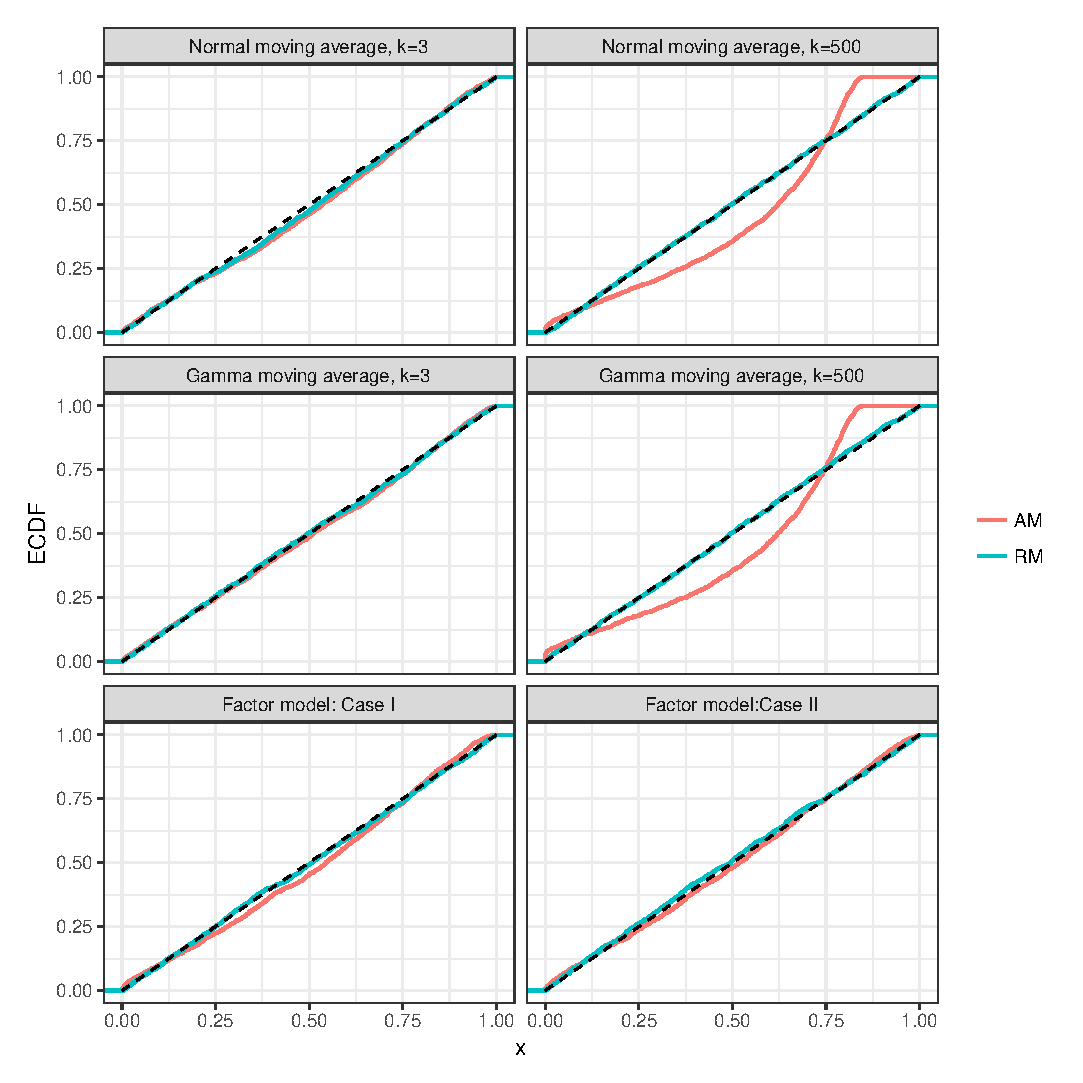
\includegraphics[ width=174mm]{pValuePlotProposed}
    \caption{The ECDF of $p$-values for the asymptotic method (AM) and the randomization method (RM).  $p=600$, $n=100$.}\label{figure:ECDF}
\end{figure*}

In Theorem~\ref{shaziCLT}, we proved that the randomization distribution tends to a standard normal distribution under certain conditions.
In Figure~\ref{figure:histogram}, we plot the histograms of the randomization distribution under null hypothesis.
For comparison, we also plot the standard normal density.
From the plots, we can see that the randomization distribution is very similar to the standard normal distribution in factor model and moving average model with $k=3$.
This verifies the Theorem~\ref{shaziCLT}.
However, under moving average model with $k=500$, the randomization distribution is far from standard normal distribution.
This implies the accuracy of normal approximation depends on the innovation model.


\begin{figure*}[htbp]
    \centering
    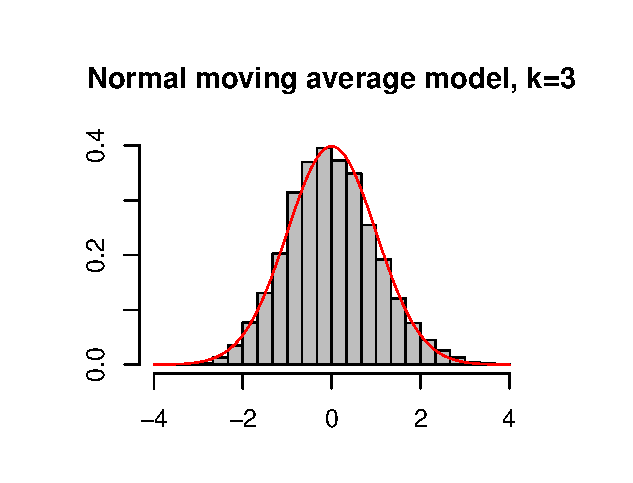
\includegraphics[width=84mm]{normal3}
    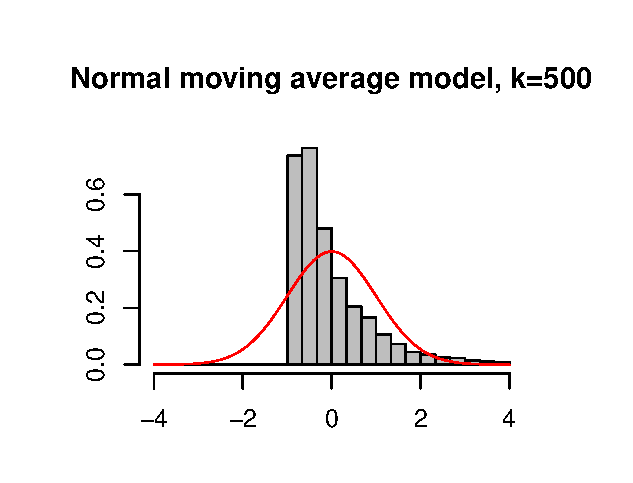
\includegraphics[width=84mm]{normal500}\\
    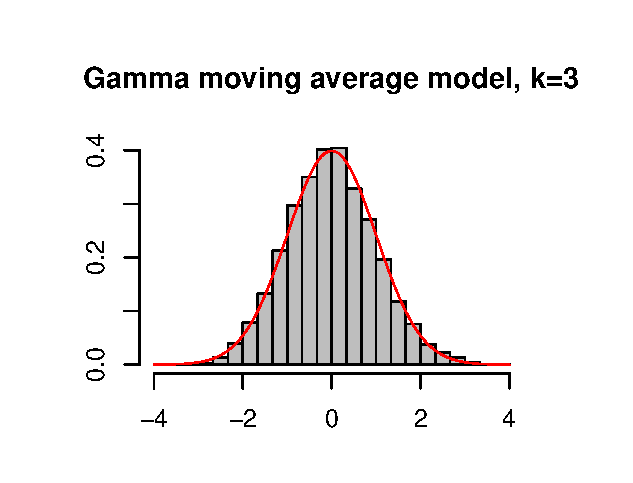
\includegraphics[width=84mm]{gamma3}
    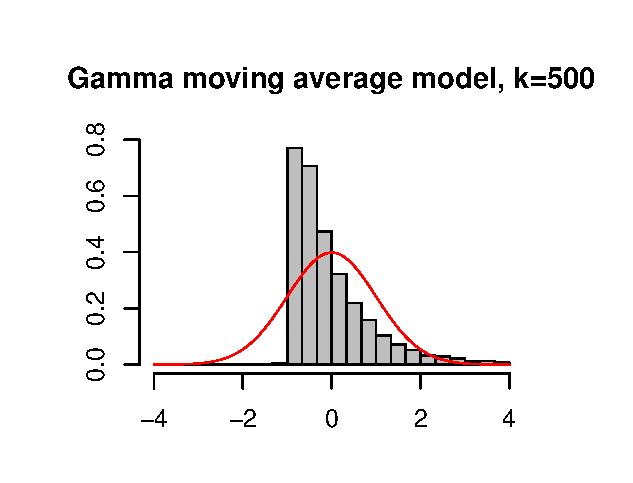
\includegraphics[width=84mm]{gamma500}\\
    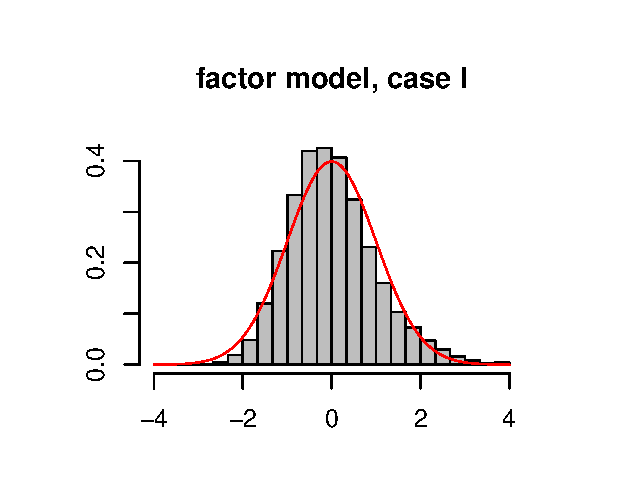
\includegraphics[width=84mm]{factor1}
    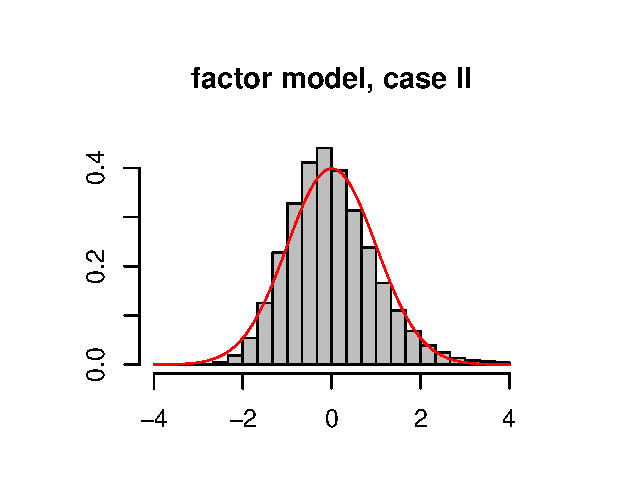
\includegraphics[width=84mm]{factor2}\\
    \caption{The histograms of the randomization distribution. $p=600$, $n=100$.}\label{figure:histogram}
\end{figure*}




Now we simulate the empirical power and size.
Let $\mathrm{SNR}=\sqrt{n(n-1)}\mu^T \mu /\sqrt{2\mytr \Sigma^2}$ be the signal to noise ratio (SNR).
The theoretic asymptotic power is an increasing function of SNR\@.
We scale $\mu$ to reach different level of SNR\@.
Our simulation consider two mean structure: dense mean and sparse mean.
In the dense mean setting, each coordinate of $\mu$ is independently generated from $U(2,3)$ and then $\mu$ is scaled to reach a given SNR\@.
In the sparse mean setting, we randomly select $5\%$ of $\mu$'s $p$ coordinates to be non-zero.
Each non-zero coordinate is again independently generated from $U(2,3)$ and then scaled to reach a given SNR\@.
We set $B=1000$ for the randomization test method.
The empirical power and size are computed based on $2000$ simulations.

Table~\ref{table1} and Table~\ref{table2} list the empirical power and size for the moving average model.
It's not surprising that the randomization test can control level well in normal case.
The results also show that the randomization method can control level well even in Gamma case, which is not symmetric under null.
It justifies the robustness of the randomization method.
On the other hand, asymptotic method has small size when the correlations between variables are weak and has inflated size when the correlations are strong.
The empirical power of the randomization method is similar to the asymptotic method.
They are both similar to theoretical asymptotic power~\eqref{oPower} when $k$ is small and are both lower than theoretical asymptotic power when $k$ is large.
Table~\ref{table3} lists the empirical power and size under factor model.
Although the distribution is not symmetric, the results show that the level of the randomization method is close to $0.05$ while asymptotic method suffers from level inflation.
In summary, the simulation results show that the randomization method is robust and has similar power with asymptotic method.

\begin{table*}[ht]
    \caption{Empirical power and size of moving average model with normal innovation.  $p=600$, $n=100$, $\alpha=0.05$. TP is the theoretical asymptotic power, RM represents the randomization method, AM represents the asymptotic method.}
\label{table1}
    \centering
    \begin{tabular}{cccccccccccc}
          \toprule
          &&& & \multicolumn{4}{c}{Dense means} &\multicolumn{4}{c}{Sparse means}\\
          \cmidrule(r){5-8}\cmidrule(r){9-12}
          &&& & \multicolumn{2}{c}{$k=3$} & \multicolumn{2}{c}{$k=500$} & \multicolumn{2}{c}{$k=3$}& \multicolumn{2}{c}{$k=500$}\\
          \cmidrule(r){5-6}  \cmidrule(r){7-8} \cmidrule(r){9-10}  \cmidrule(r){11-12}
           $n$&$p$&SNR& TP & RM & AM & RM & AM & RM & AM & RM & AM  \\ 
            \midrule
        100&600&0.0 & 0.050 & 0.0445 & 0.0515 & 0.0530 & 0.0745 & 0.0500 & 0.0585 & 0.0515 & 0.0715 \\ 
          &&0.5 & 0.126 & 0.1815 & 0.1940 & 0.1330 & 0.1685 & 0.1735 & 0.1875 & 0.0780 & 0.1130 \\ 
            &&1.0 & 0.260 & 0.4075 & 0.4295 & 0.2250 & 0.2785 & 0.4060 & 0.4325 & 0.1505 & 0.2065 \\ 
              &&1.5 & 0.442 & 0.6295 & 0.6535 & 0.3435 & 0.3920 & 0.6520 & 0.6755 & 0.2480 & 0.3355 \\ 
                &&2.0 & 0.639 & 0.7895 & 0.8055 & 0.3935 & 0.4665 & 0.8575 & 0.8765 & 0.3850 & 0.5400 \\ 
                  &&2.5 & 0.804 & 0.9165 & 0.9215 & 0.4775 & 0.5425 & 0.9655 & 0.9695 & 0.6355 & 0.8155 \\ 
                    &&3.0 & 0.912 & 0.9640 & 0.9695 & 0.5445 & 0.6090 & 0.9910 & 0.9935 & 0.8720 & 0.9730 \\ 
% new simulations
        200&1000&0.0 & 0.050 & 0.0505 & 0.0550 & 0.0505 & 0.0695 & 0.0520 & 0.0575 & 0.0510 & 0.0700 \\ 
          &&0.5 & 0.126 & 0.1885 & 0.2025 & 0.1410 & 0.1680 & 0.1745 & 0.1865 & 0.0855 & 0.1165 \\ 
            &&1.0 & 0.260 & 0.3875 & 0.4050 & 0.2090 & 0.2620 & 0.4010 & 0.4160 & 0.1485 & 0.2075 \\ 
              &&1.5 & 0.442 & 0.6425 & 0.6600 & 0.3180 & 0.3715 & 0.6725 & 0.6895 & 0.2355 & 0.3290 \\ 
                &&2.0 & 0.639 & 0.8245 & 0.8355 & 0.4210 & 0.4760 & 0.8710 & 0.8845 & 0.3855 & 0.5310 \\ 
                  &&2.5 & 0.804 & 0.9210 & 0.9265 & 0.4885 & 0.5475 & 0.9690 & 0.9710 & 0.6290 & 0.8050 \\ 
                    &&3.0 & 0.912 & 0.9820 & 0.9830 & 0.6045 & 0.6530 & 0.9940 & 0.9960 & 0.8670 & 0.9780 \\ 
        \bottomrule
    \end{tabular}
\end{table*}

\begin{table*}[ht]
    \caption{Empirical power and size of moving average model with Gamma innovation.  $p=600$, $n=100$, $\alpha=0.05$. TP is the theoretical asymptotic power, RM represents the randomization method, AM represents the asymptotic method.}
\label{table2}
    \centering
    \begin{tabular}{cccccccccccc}
          \toprule
          &&& & \multicolumn{4}{c}{Dense means} &\multicolumn{4}{c}{Sparse means}\\
          \cmidrule(r){5-8}\cmidrule(r){9-12}
          &&& & \multicolumn{2}{c}{$k=3$} & \multicolumn{2}{c}{$k=500$} & \multicolumn{2}{c}{$k=3$}& \multicolumn{2}{c}{$k=500$}\\
          \cmidrule(r){5-6}  \cmidrule(r){7-8} \cmidrule(r){9-10}  \cmidrule(r){11-12}
           $n$&$p$&SNR& TP & RM & AM & RM & AM & RM & AM & RM & AM \\ 
            \midrule
        100&600&0.0 & 0.050 & 0.0450 & 0.0550 & 0.0475 & 0.0660 & 0.0405 & 0.0465 & 0.0505 & 0.0765 \\ 
          &&0.5 & 0.126 & 0.1815 & 0.1975 & 0.1365 & 0.1750 & 0.1765 & 0.1870 & 0.0985 & 0.1345 \\ 
            &&1.0 & 0.260 & 0.3825 & 0.4050 & 0.2375 & 0.2765 & 0.4130 & 0.4335 & 0.1550 & 0.2070 \\ 
              &&1.5 & 0.442 & 0.6210 & 0.6465 & 0.2975 & 0.3490 & 0.6580 & 0.6745 & 0.2225 & 0.3135 \\ 
                &&2.0 & 0.639 & 0.8180 & 0.8325 & 0.3920 & 0.4450 & 0.8645 & 0.8800 & 0.3890 & 0.5340 \\ 
                  &&2.5 & 0.804 & 0.9115 & 0.9260 & 0.4900 & 0.5465 & 0.9635 & 0.9665 & 0.6280 & 0.8200 \\ 
                    &&3.0 & 0.912 & 0.9710 & 0.9765 & 0.5505 & 0.6085 & 0.9940 & 0.9945 & 0.8600 & 0.9740 \\ 
% new simulation
                   200 & 1000 &0.0 & 0.050 & 0.0520 & 0.0555 & 0.0495 & 0.0715 & 0.0505 & 0.0555 & 0.0455 & 0.0690 \\ 
                      &&0.5 & 0.126 & 0.1740 & 0.1880 & 0.1355 & 0.1725 & 0.1725 & 0.1840 & 0.0780 & 0.1170 \\ 
                        &&1.0 & 0.260 & 0.3890 & 0.4045 & 0.2175 & 0.2595 & 0.4220 & 0.4415 & 0.1475 & 0.1950 \\ 
                          &&1.5 & 0.442 & 0.6470 & 0.6630 & 0.3240 & 0.3820 & 0.6605 & 0.6855 & 0.2550 & 0.3375 \\ 
                            &&2.0 & 0.639 & 0.8175 & 0.8285 & 0.4180 & 0.4755 & 0.8580 & 0.8750 & 0.3835 & 0.5205 \\ 
                              &&2.5 & 0.804 & 0.9295 & 0.9335 & 0.4870 & 0.5560 & 0.9600 & 0.9645 & 0.6075 & 0.7970 \\ 
                                &&3.0 & 0.912 & 0.9755 & 0.9765 & 0.5865 & 0.6505 & 0.9915 & 0.9935 & 0.8760 & 0.9790 \\ 
        \bottomrule
    \end{tabular}
\end{table*}

\begin{table*}[ht]
    \caption{Empirical power and size of factor model innovation.  $p=600$, $n=100$, $\alpha=0.05$. TP is the theoretical asymptotic power, RM represents the randomization method, AM represents the asymptotic method.}
\label{table3}
    \centering
    \begin{tabular}{cccccccccccc}
          \toprule
          &&& & \multicolumn{4}{c}{Dense means} &\multicolumn{4}{c}{Sparse means}\\
          \cmidrule(r){5-8}\cmidrule(r){9-12}
          &&& & \multicolumn{2}{c}{Case I} & \multicolumn{2}{c}{Case II} & \multicolumn{2}{c}{Case I}& \multicolumn{2}{c}{Case II}\\
          \cmidrule(r){5-6}  \cmidrule(r){7-8} \cmidrule(r){9-10}  \cmidrule(r){11-12}
           $n$&$p$&SNR& TP & RM & AM & RM & AM & RM & AM & RM & AM  \\ 
            \midrule
        100&600&0.0 & 0.050 & 0.0465 & 0.0610 & 0.0455 & 0.0590 & 0.0475 & 0.0625 & 0.0505 & 0.0615 \\ 
          &&0.5 & 0.126 & 0.1315 & 0.1555 & 0.1465 & 0.1650 & 0.1200 & 0.1380 & 0.1080 & 0.1320 \\ 
            &&1.0 & 0.260 & 0.2420 & 0.2780 & 0.2550 & 0.2780 & 0.1940 & 0.2250 & 0.2075 & 0.2400 \\ 
              &&1.5 & 0.442 & 0.3635 & 0.3975 & 0.3555 & 0.3870 & 0.3670 & 0.4110 & 0.3740 & 0.4155 \\ 
                &&2.0 & 0.639 & 0.4825 & 0.5165 & 0.4720 & 0.4975 & 0.5340 & 0.5930 & 0.5615 & 0.6015 \\ 
                  &&2.5 & 0.804 & 0.5860 & 0.6190 & 0.5825 & 0.6165 & 0.7040 & 0.7610 & 0.7120 & 0.7505 \\ 
                    &&3.0 & 0.912 & 0.6730 & 0.7060 & 0.6975 & 0.7210 & 0.8525 & 0.8815 & 0.8680 & 0.8920 \\ 
        200&1002&0.0 & 0.050 & 0.0520 & 0.0670 & 0.0530 & 0.0665 & 0.0485 & 0.0615 & 0.0490 & 0.0615 \\ 
          &&0.5 & 0.126 & 0.1490 & 0.1895 & 0.1405 & 0.1675 & 0.0905 & 0.1115 & 0.0975 & 0.1230 \\ 
            &&1.0 & 0.260 & 0.2450 & 0.2780 & 0.2485 & 0.2785 & 0.1835 & 0.2330 & 0.1920 & 0.2305 \\ 
              &&1.5 & 0.442 & 0.3445 & 0.3915 & 0.3450 & 0.3745 & 0.3170 & 0.3745 & 0.3395 & 0.3935 \\ 
                &&2.0 & 0.639 & 0.4605 & 0.5035 & 0.4775 & 0.5170 & 0.5080 & 0.5995 & 0.5365 & 0.5925 \\ 
                  &&2.5 & 0.804 & 0.5355 & 0.5810 & 0.5900 & 0.6320 & 0.7040 & 0.7775 & 0.7345 & 0.7850 \\ 
                    &&3.0 & 0.912 & 0.6280 & 0.6640 & 0.6660 & 0.6960 & 0.8670 & 0.9115 & 0.8655 & 0.9070 \\ 
        \bottomrule
    \end{tabular}
\end{table*}

%\subsection{The second simulation study}
%The computation of our randomization test is easy since we only need to compute $X_i^T X_j$ once, $1\leq j<i \leq n$.
%The same technique can be applied to the statistic $\sum_{i\neq j}\|X_i\|^{-1}\|X_j\|^{-1}X_i^T X_j$ in~\cite{Wang2015A}.
%However, the technique can not be applied to the statistic $\bar{X}^T [\mydiag(S)]^{-1}\bar{X}$ in~\cite{Srivastava2008A} and the statistic $\bar{X}^T (I_p-\BP_S)\bar{X}$ in~\cite{Zhao2016A}.
%Generally, many high dimensional test statistics for hypotheses~\eqref{ourHy} can be written as generalized quadratic forms of data
%$$
%\sum_{i=1}^n \sum_{j=1}^n X_i^T A X_j,
%$$
%Where $A$ is a $p\times p$ matrix which only depends on $S$.
%The difficulty is that for each randomization, the matrix $A$ should be recalculated.
%It consumes a lot time.
%However, 
%the matrix $A$ is used to estimate the structure of $\Sigma$, which should not change during randomization.
%This motivates us to hold $A$ constant during randomization.
%More precisely, for a randomization, we generate $\epsilon_1,\ldots,\epsilon_n$ and compute
%$$
%\sum_{j<i} X_i^T A X_j \epsilon_i \epsilon_j.
%$$
%We simulate the level.
%
%We consider the following $A$:
%$A_1=[\mydiag(S)]^{-1}$,
%$A_2=\bar{X} S^{+}\bar{X}$,
%$A_3=(I-\BP_S)$,
%$A_4=S$.







\section{Conclusion Remark}
In this paper, we considered a randomization test for mean vector in high dimensional setting.
A fast implementation was provided.
We also derived some asymptotic properties of the test procedure.
 In fact, the algorithm and the proof method can also be applied to other quadratic based statistics.

We showed that even if the symmetric assumption is violated, the randomization test also has correct level asymptotically.
Hence the test procedure is robust.
%It is interesting to investigate the robustness of randomization test in finite sample case.

In classical statistics, randomization test procedures are time consuming.
Nevertheless, the computational complexity of our randomization test procedure is not affected by the data dimension $p$. 
Hence we have reason to believe that randomization tests may be generally suitable for high dimensional problems.


Maybe the most widely used randomization method is the two sample permutation test.
As~\citet{Romano1990On} pointed out, the asymptotic property of randomization tests depends heavily on the particular problem and the two sample case is quite distinct from the one sample case.
The method used in this paper can not be applied to permutation test.
We leave this problem for further work.


\section*{Appendix}
\paragraph{A CLT for quadratic form of Rademacher variables}
The proof of the Theorem~\ref{shaziCLT} is based on a CLT of the quadratic form of Rademacher variables. 
Such a CLT can be also used to study the asymptotic behavior of many other randomization test.
 Let $\epsilon_1,\ldots,\epsilon_n$ be independent Rademacher  variables. 
 Consider the quadratic form $W_n=\sum_{1\leq j<i\leq n} a_{ij}\epsilon_i \epsilon_j$, where $\{a_{ij}\}$ are nonrandom numbers. Here $\{\epsilon_i\}$ and $\{a_{ij}\}$ may depend on $n$, a parameter we suppress.
 By direct calculation, we have $\myE(W_n)=0$ and $\mathrm{Var}(W_n)=\sum_{1\leq j<i\leq n} a_{ij}^2$.

 \begin{proposition}\label{CLTprop}
     A sufficient condition for
     \begin{equation*}
         \frac{W_n}{\sqrt{\sum_{1\leq j<i\leq n} a_{ij}^2}}\xrightarrow{\mathcal{L}} N(0,1)
     \end{equation*}
     is that
     \begin{equation*}
         \sum_{j<k}{(\sum_{i:i>k}a_{ij}a_{ik})}^2+
         \sum_{j<i}a_{ij}^4+
         \sum_{j<k<i}a_{ij}^2 a_{ik}^2
         =o\big({(\sum_{j<i} a_{ij}^2)}^2\big).
     \end{equation*}
 \end{proposition}

 \begin{proof}
     Note that we have the decomposition $W_n=\sum_{i=2}^n U_{in}$, where $U_{in} =\epsilon_i \sum_{j=1}^{i-1} a_{ij}\epsilon_j$, $i=2,\ldots,n$.
    Let $\mathcal{F}_{in}$ be the $\sigma$-field generated by $\epsilon_1,\ldots,\epsilon_i$, $i=1,\ldots, n$.
     Then it can be seen that $\{U_{in}\}_{i=1}^n$
       is a martingale difference array with respect to $\{\mathcal{F}_{in}\}_{i=1}^n$. 
     Hence the martingale central limit theorem can be used. See, for example,~\citet[Theorem 1 of Chapter VIII ]{pollard1984convergence}.
     By martingale central limit theorem, our conclusion holds if the following two conditions are satisfied:
     \begin{equation}\label{MCLTcondition1}
         \frac{\sum_{i=2}^n \myE(U_{in}^2 |\mathcal{F}_{i-1,n})}{\sum_{1\leq j<i\leq n} a_{ij}^2}\xrightarrow{P} 1,
     \end{equation}
     and
     \begin{equation}\label{MCLTcondition2}
         \frac{\sum_{i=2}^n \myE\big(U_{in}^2\big\{U_{in}^2>\epsilon \sum_{1\leq j<i\leq n} a_{ij}^2\big\}\big|\mathcal{F}_{i-1,n}\big)}{\sum_{1\leq j<i\leq n} a_{ij}^2}\xrightarrow{P} 0,
     \end{equation}
     for every $\epsilon>0$.

     \paragraph{Proof of~\eqref{MCLTcondition1}}
     Since $\myE(U_{in}^2 |\mathcal{F}_{i-1,n})={(\sum_{j=1}^{i-1}a_{ij}\epsilon_j)}^2$, we have that
     \begin{equation*}
         \begin{aligned}
             &\sum_{i=2}^n \myE(U_{in}^2 |\mathcal{F}_{i-1,n})
             =\sum_{i=2}^n \big(\sum_{j=1}^{i-1}a_{ij}\epsilon_j \big)^2\\
             =&\sum_{i=2}^n \big( \sum_{j=1}^{i-1} a_{ij}^2 +2\sum_{j,k:j<k<i} a_{ij}a_{ik}\epsilon_j \epsilon_k \big)\\
             =&\sum_{i=2}^n  \sum_{j=1}^{i-1} a_{ij}^2 +2\sum_{j<k<i} a_{ij}a_{ik}\epsilon_j \epsilon_k.
         \end{aligned}
     \end{equation*}
     For the second term, we have that
     \begin{equation*}
         \begin{aligned}
             &\myE{(\sum_{j<k<i} a_{ij}a_{ik}\epsilon_j \epsilon_k)}^2
             =
             \myE{\big(\sum_{j<k} (\sum_{i:i>k}a_{ij}a_{ik})\epsilon_j \epsilon_k \big)}^2\\
             =&
             \sum_{j<k} (\sum_{i:i>k}a_{ij}a_{ik})^2
             =
             o\big({(\sum_{j<i} a_{ij}^2)}^2\big),
         \end{aligned}
     \end{equation*}
     where the last equality holds by assumption.
     Then it follows that
     \begin{equation*}
         \frac{\sum_{j<k<i} a_{ij}a_{ik}\epsilon_j \epsilon_k}{\sum_{j<i} a_{ij}^2}\xrightarrow{P} 0.
     \end{equation*}
     Hence~\eqref{MCLTcondition1} holds.
     \paragraph{Proof of~\eqref{MCLTcondition2}}
     By Markov inequality, it's sufficient to prove
     \begin{equation}\label{temp1}
         \frac{\sum_{i=2}^n \myE\big(U_{in}^4\big|\mathcal{F}_{i-1,n}\big)}{{\big(\sum_{1\leq j<i\leq n} a_{ij}^2\big)}^2}\xrightarrow{P} 0.
     \end{equation}
     Since the relevant random variables are all positive, we only need to prove~\eqref{temp1} converges to $0$ in mean. But
     \begin{equation*}
         \begin{aligned}
             &\sum_{i=2}^n \myE U_{in}^4
             =
             \sum_{i=2}^n \myE {(\sum_{j:j<i}a_{ij}\epsilon_j)}^4\\
             =&
             \sum_{i=2}^n \myE {(\sum_{j:j<i}a_{ij}^2+2\sum_{j,k:j<k<i}a_{ij}a_{ik}\epsilon_j \epsilon_k)}^2\\
             =&
             \sum_{i=2}^n  \big({(\sum_{j:j<i}a_{ij}^2)}^2+4\myE{(\sum_{j,k:j<k<i}a_{ij}a_{ik}\epsilon_j \epsilon_k)}^2 \big)\\
             =&
             \sum_{i=2}^n  (\sum_{j:j<i}a_{ij}^4+6\sum_{j,k:j<k<i}a_{ij}^2 a_{ik}^2)\\
             =&
             \sum_{j<i}a_{ij}^4+6\sum_{j<k<i}a_{ij}^2 a_{ik}^2
             =
             o\big({(\sum_{j<i} a_{ij}^2)}^2\big),
         \end{aligned}
     \end{equation*}
     where the last equality holds by assumption. Hence~\eqref{MCLTcondition2} holds.
 \end{proof}

The rest of Appendix is devoted to the proof of our main results.



\begin{lemma}\label{lemmaUniformSimple}
    Suppose $\{\eta_n\}_{n=1}^{\infty}$ is a sequence of random variables, weakly converges to $\eta$, a random variable with continuous distribution function.
    Then we have
    $$
    \sup_{x}|\Pr(\eta_n\leq x)-\Pr(\eta\leq x)|\to 0.
    $$
\end{lemma}

For two non-negative sequences $\{x_n\}_{n=1}^{\infty}$ and $\{y_n\}_{n=1}^{\infty}$, we write $a_n\asymp b_n$ to denote 
$$cb_n\leq a_n\leq C b_n$$
for some absolute constants $c>0$, $C>0$ and all $n=1,2,\ldots$.
\begin{lemma}\label{lemmaQ}
    Under~\eqref{chenC2}, suppose $A=(a_{ij})$ is an $m\times m$ positive semi-definite matrix, we have
        $$
        \myE {(Z_i^T A Z_i)}^2\asymp {(\mytr A)}^2.
        $$
\begin{proof}
Notice that
    $$
    \begin{aligned}
        &{(Z_i^T A Z_i)}^2
        =
        (\sum_{j=1}^m a_{jj}z_{ij}^2+2\sum_{k<j}a_{jk}z_{ij}z_{ik})^2\\
        =&
        (\sum_{j=1}^m a_{jj}z_{ij}^2)^2+
        4(\sum_{j=1}^m a_{jj}z_{ij}^2)(\sum_{k<j}a_{jk}z_{ij}z_{ik})\\
        &+
        4(\sum_{k<j}a_{jk}z_{ij}z_{ik})^2\\
        =&
        \sum_{j=1}^m a_{jj}^2z_{ij}^4+2\sum_{k<j}a_{jj}a_{kk}z_{ij}^2 z_{ik}^2+
        4(\sum_{j=1}^m a_{jj}z_{ij}^2)(\sum_{k<j}a_{jk}z_{ij}z_{ik})\\
        &+
        4\Big(\sum_{k<j}a_{jk}^2z_{ij}^2z_{ik}^2\\
        &+\sum_{k<j,l<\alpha:\mathrm{card}(\{k,j\}\cap\{l,\alpha\})<2} a_{jk}a_{\alpha l}z_{ij}z_{ik}z_{i\alpha}z_{il}\Big),
    \end{aligned}
    $$
    where $\mathrm{card}(\cdot)$ is the cardinality of a set.
    By the assumption~\eqref{chenC2}, we have
    $$
    \begin{aligned}
        &\myE{(Z_i^T A Z_i)}^2\\
        =&
        \sum_{j=1}^n a_{jj}^2 \myE z_{ij}^4+2\sum_{k<j}a_{jj}a_{kk}\myE(z_{ij}^2 z_{ik}^2)+
        4\sum_{k<j}a_{jk}^2 \myE(z_{ij}^2z_{ik}^2)\\
        \asymp &
        \sum_{j=1}^n\sum_{k=1}^n a_{jj}a_{kk}+
        \sum_{j=1}^n\sum_{k=1}^n a_{jk}^2
        ={(\mytr (A))}^2+\mytr ( A^2).
    \end{aligned}
    $$

     Then the conclusion holds from inequality
     $$\mytr ( A^2)\leq \lambda_1 (A) \mytr(A)\leq {(\mytr A)}^2.$$

\end{proof}
\end{lemma}

\begin{lemma}\label{smallLemma1}
    Under~\eqref{chenC1} and~\eqref{chenC2}, for $i\neq j$ we have
    \begin{equation}\label{eq:20170220}
        \myE{(X_i^T X_j)}^4=%O\Big({\big(\mytr (\Sigma+\mu\mu^T)^2\big)}^2\Big).
             O(1){\Big(\mytr {\big(\Sigma+\mu\mu^T\big)}^2\Big)}^2.
    \end{equation}
\end{lemma}
\begin{proof}

    Under~\eqref{chenC1} and~\eqref{chenC2}, we have
    $$
        \begin{aligned}
            &{(X_i^T X_j)}^4=
            {(Z_i^T \Gamma^T \Gamma Z_j+\mu^T \Gamma Z_i+\mu^T \Gamma Z_j+\mu^T \mu)}^4\\
            \leq &
            64\big((Z_i^T \Gamma^T \Gamma Z_j)^4+(\mu^T \Gamma Z_i)^4+(\mu^T \Gamma Z_j)^4+(\mu^T \mu)^4\big)\\
        \end{aligned}
    $$
    We can deal with the first term by applying Lemma~\ref{lemmaQ} twice:
        $$
        \begin{aligned}
            &\myE(Z_i^T \Gamma^T \Gamma Z_j)^4=
        \myE(Z_i^T \Gamma^T \Gamma Z_j Z_j^T \Gamma^T \Gamma Z_i)^2\\
            =&
            \myE\myE\big((Z_i^T \Gamma^T \Gamma Z_j Z_j^T \Gamma^T \Gamma Z_i)^2 | Z_j\big)\\
            \asymp &  \myE{(Z_j^T \Gamma^T \Sigma \Gamma Z_j)}^2
            \asymp   {\big(\mytr (\Sigma^2)\big)}^2.%+\mytr \Sigma^4\\
            %\leq &  (\mytr \Sigma^2)^2+\lambda_{1}^2(\Sigma)\mytr \Sigma^2,
        \end{aligned}
    $$
    Similarly, we have
        $$
        \begin{aligned}
            &\myE(\mu^T \Gamma Z_i)^4=
        \myE(Z_i^T \Gamma^T \mu\mu^T \Gamma Z_i)^2
            \asymp  {(\mu^T \Sigma \mu)}^2\\
            &\leq \lambda_{1}^2(\Sigma){(\mu^T \mu)}^2
        \leq \mytr (\Sigma^2){(\mu^T \mu)}^2
            \leq {\big(\mytr (\Sigma^2)\big)}^2+{(\mu^T \mu)}^4.
        %\leq \lambda_{1}^2(\Sigma){(\mu^T\mu)}^2
        \end{aligned}
    $$
Hence
$$
    \myE (X_i^T X_j)^4=O(1)\Big(\big(\mytr(\Sigma^2)\big)^2+(\mu^T \mu)^4\Big).
    $$
Then the theorem follows by noting that
$$
{\Big(\mytr {\big(\Sigma+\mu\mu^T\big)}^2\Big)}^2
\asymp
    \big(\mytr(\Sigma^2)\big)^2+(\mu^T \mu)^4.
$$
\end{proof}


\begin{lemma}\label{smallLemma2}
    Under~\eqref{chenC1},~\eqref{chenC2}, suppose $i\neq j$, $i\neq k$, $j\neq k$, we have
    \begin{equation}\label{eq:2}
            \myE{(X_i^T X_j)}^2{(X_k^T X_i)}^2=
             O(1){\Big(\mytr {\big(\Sigma+\mu\mu^T\big)}^2\Big)}^2.
    \end{equation}
\end{lemma}
\begin{proof}
Note that
    \begin{equation*}
        \begin{aligned}
            &\myE{(X_i^T X_j)}^2{(X_k^T X_i)}^2
            = 
            \myE\myE\big({(X_i^T X_j)}^2{(X_k^T X_i)}^2| X_i\big)\\
            =&
            \myE{(X_i^T (\Sigma+\mu\mu^T) X_i )}^2\\
            =&
            \myE\Big(Z_i^T \Gamma^T (\Sigma+\mu\mu^T) \Gamma Z_i+ 2\mu^T (\Sigma+\mu\mu^T)\Gamma Z_i \\
            &+\mu^T \Sigma \mu +(\mu^T\mu)^2 \Big)^2\\
            \leq&
            4\myE(Z_i^T \Gamma^T (\Sigma+\mu\mu^T) \Gamma Z_i)^2+ 16\myE(\mu^T (\Sigma+\mu\mu^T)\Gamma Z_i)^2 \\
            &+4(\mu \Sigma \mu)^2 +4(\mu^T\mu)^4.
        \end{aligned}
    \end{equation*}
    By Lemma~\eqref{lemmaQ}, we have
    \begin{equation*}
        \begin{aligned}
            &\myE(Z_i^T \Gamma^T (\Sigma+\mu\mu^T) \Gamma Z_i)^2\\
            \asymp&
\big(\mytr (\Gamma^T (\Sigma+\mu\mu^T)\Gamma)\big)^2\\
            =&
\big(\mytr \Sigma^2+\mu^T\Sigma \mu\big)^2\\
            \leq&
            2{\big(\mytr \Sigma^2\big)}^2+2{\big(\mu^T\Sigma \mu\big)}^2.
        \end{aligned}
    \end{equation*}
    On the other hand, we have
    \begin{equation*}
        \begin{aligned}
            &\myE(\mu^T (\Sigma+\mu\mu^T)\Gamma Z_i)^2\\
            =&
\mu^T (\Sigma+\mu\mu^T)\Sigma (\Sigma+\mu\mu^T)\mu\\
            =&\mu^T \Sigma^3 \mu+2(\mu^T\mu)(\mu^T\Sigma^2\mu)+{(\mu^T\mu)}^2(\mu^T\Sigma\mu).
        \end{aligned}
    \end{equation*}
    For $i=1,2,3$, we have
    $$
    \mu^T \Sigma^i \mu
    \leq \lambda_{1}^i(\Sigma)\mu^T\mu
    \leq {(\mytr (\Sigma^2))}^{i/2}\mu^T\mu.
    $$
        Combining these yields
        $$
        \begin{aligned}
            &\myE{(X_i^T X_j)}^2{(X_k^T X_i)}^2\\
            =&
            O(1)\Big({\big(\mytr (\Sigma^2)\big)}^2+
            {\big(\mytr (\Sigma^2)\big)}^{3/2}\mu^T \mu+
            {\big(\mytr (\Sigma^2)\big)}{(\mu^T \mu)}^2\\
            &+
            {\big(\mytr (\Sigma^2)\big)}^{1/2}{(\mu^T \mu)}^3+
            {(\mu^T \mu)}^4
            \Big)\\
            =&O(1)
            \Big(\big(\mytr(\Sigma^2)\big)^2 + (\mu^T \mu)^4 \Big)\\
            =& O(1){\Big(\mytr {\big(\Sigma+\mu\mu^T\big)}^2\Big)}^2.
        \end{aligned}
        $$
\end{proof}


\begin{lemma}\label{ratioLemma}
    Under~\eqref{chenC1} and~\eqref{chenC2}, we have
        $$
        \frac{\sum_{j<i}{(X_i^T X_j)}^2}{\frac{n(n-1)}{2}\mytr  (\Sigma+\mu\mu^T)^2}
        \xrightarrow{P}1.
        $$
\end{lemma}
\begin{proof}
    Since
        $$
        \begin{aligned}
            \myE(X_i^T X_j)^2=&
            \myE(X_i^T X_j X_j^T X_i)=
            \myE(X_i^T (\Sigma+\mu \mu^T) X_i)\\
            =&
            \myE\mytr ((\Sigma+\mu \mu^T) X_i X_i^T)=\mytr {(\Sigma+\mu \mu^T)}^2,
        \end{aligned}
    $$
   we have 
        $$
        \myE\sum_{j<i}(X_i^T X_j)^2=\frac{n(n-1)}{2}\mytr {(\Sigma+\mu\mu^T)}^2.
    $$
    Next we need to deal with $\myE \big(\sum_{j<i}{(X_i^T X_j)}^2\big)^2$.
    Write 
$$
    \big(\sum_{j<i}{(X_i^T X_j)}^2\big)^2=
    \big(\sum_{j<i}{(X_i^T X_j)}^2\big)
    \big(\sum_{k<l}{(X_l^T X_k)}^2\big)
    $$
    According to $\mathrm{card}(\{i,j\}\cap\{k,l\})=0,1,2$, we have
    \begin{equation*}%\label{eq:1}
    \begin{aligned}
        \big(\sum_{j<i}{(X_i^T X_j)}^2\big)^2
        &=
        \sum_{j<i}{(X_i^T X_j)}^4\\
        & +
        \sum_{j<i,k<l:\{i,j\}\cap \{k,l\}=\phi}{(X_i^T X_j)}^2{(X_l^T X_k)}^2\\
        +2\sum_{j<i<k}&\Big(
        {(X_i^T X_j)}^2{(X_k^T X_i)}^2+
{(X_i^T X_j)}^2{(X_k^T X_j)}^2\\
        &+
{(X_k^T X_j)}^2{(X_k^T X_i)}^2
        \Big).
    \end{aligned}
    \end{equation*}
    %For the three summations on the right hand side of equation~\eqref{eq:1},
    There are $n(n-1)/2$, $n(n-1)(n-2)(n-3)/4$ and $n(n-1)(n-2)/6$ terms in each sum, respectively.
    This, combined with Lemma~\ref{smallLemma1} and Lemma~\ref{smallLemma2}, yields
    $$
    \begin{aligned}
        &\myE{\big(\sum_{j<i}{(X_i^T X_j)}^2\big)}^2\\
            =&\frac{n(n-1)(n-2)(n-3)}{4}{\big(\mytr (\Sigma+\mu\mu^T)^2\big)}^2\\
            &+O(1)(\frac{n(n-1)}{2}+n(n-1)(n-2)){\big(\mytr (\Sigma+\mu\mu^T)^2\big)}^2.
    \end{aligned}
    $$
Hence we have
    \begin{equation*}
    \begin{aligned}
        &\frac{
        \mathrm{Var}(\sum_{j<i}{(X_i^T X_j)}^2)
    }{\big(\myE\sum_{j<i}{(X_i^T X_j)}^2\big)^2}\\
        =&
    \frac{
        \myE{\big(\sum_{j<i}{(X_i^T X_j)}^2\big)}^2-
        {\big(\myE\sum_{j<i}{(X_i^T X_j)}^2\big)}^2
    }{
        {\big(\myE\sum_{j<i}{(X_i^T X_j)}^2\big)}^2
    }
    =O(\frac{1}{n}).
    \end{aligned}
    \end{equation*}
    This implies 
        $$
        \frac{
        \sum_{j<i}{(X_i^T X_j)}^2
    }{\myE\sum_{j<i}{(X_i^T X_j)}^2}\xrightarrow{P}1.
    $$
    The proof is complete.
\end{proof}

\begin{lemma}
    Under~\eqref{chenC1},~\eqref{chenC2},~\eqref{chenC3} and~\eqref{mu2},
    %\begin{equation}\label{myLoc}
        %\mu^T \mu=o(\sqrt{\mytr \Sigma^2}),
    %\end{equation}
we have
    \begin{equation}\label{lemma2R1}
        \sum_{j<k}{(\sum_{i:i>k}X_i^T X_j X_i^T X_k)}^2
        =o_P\Big(\big(\frac{n(n-1)}{2}\mytr (\Sigma+\mu\mu^T)^2\big)^2\Big).
    \end{equation}
    \begin{equation}\label{lemma2R2}
        \sum_{j<k}{(X_i^T X_j)}^4=o_P\Big(\big(\frac{n(n-1)}{2}\mytr (\Sigma+\mu\mu^T)^2\big)^2\Big)
    \end{equation}
    \begin{equation}\label{lemma2R3}
        \sum_{j<k<i}{(X_i^T X_j)}^2{(X_i^T X_k)}^2 =o_P\Big(\big(\frac{n(n-1)}{2}\mytr (\Sigma+\mu\mu^T)^2\big)^2\Big)
    \end{equation}
\end{lemma}
\begin{proof}
    We have
    \begin{equation*}
    \begin{aligned}
        &\myE\sum_{j<k}{(\sum_{i:i>k}X_i^T X_j X_i^T X_k)}^2\\
        =&
        \myE\sum_{j<k}\Big(\sum_{i:i>k}(X_i^T X_j)^2 (X_i^T X_k)^2\\
        &+2\sum_{i_1,i_2:i_1>i_2>k}X_{i_1}^T X_j X_{i_1}^T X_k X_{i_2}^T X_j X_{i_2}^T X_k\Big)\\
        =&
        \myE\sum_{j<k<i}(X_i^T X_j)^2 (X_i^T X_k)^2\\
        &+2\myE\sum_{j<k<i_2<i_1}X_{i_1}^T X_j X_{i_1}^T X_k X_{i_2}^T X_j X_{i_2}^T X_k.\\
    \end{aligned}
    \end{equation*}
    By Lemma~\ref{smallLemma1}, we have
    \begin{equation*}
    \begin{aligned}
        \myE\sum_{j<k<i}(X_i^T X_j)^2 (X_i^T X_k)^2    =O(n^3)\big(\mytr (\Sigma+\mu\mu^T)^2\big)^2.
    \end{aligned}
    \end{equation*}
And
    \begin{equation*}
    \begin{aligned}
        &\myE\sum_{j<k<i_2<i_1}X_{i_1}^T X_j X_{i_1}^T X_k X_{i_2}^T X_j X_{i_2}^T X_k\\
        =&\frac{n(n-1)(n-2)(n-3)}{6}\mytr {(\Sigma+\mu\mu^T)}^4\\
        \leq& \frac{n(n-1)(n-2)(n-3)}{6}8(\mytr (\Sigma^4)+(\mu^T \mu)^4)\\
        \leq& O(n^4)(\lambda_{1}^2(\Sigma)\mytr (\Sigma^2)+(\mu^T \mu)^4)\\
        =&
        o\Big(n^4{\big(\mytr (\Sigma^2)\big)}^2\Big),
    \end{aligned}
    \end{equation*}
    where the last line follows by assumption~\eqref{chenC3} and~\eqref{mu2}.
    This proves~\eqref{lemma2R1}. And~\eqref{lemma2R2} and~\eqref{lemma2R3} follow by Lemma~\ref{smallLemma1} and Lemma~\ref{smallLemma2}, respectively.

\end{proof}

\textbf{Proof of Theorem~\ref{shaziCLT}}

\begin{proof}
By a standard subsequence argument, we only need to prove 
    \begin{equation}\label{changchuan}
        \begin{aligned}
            &\rho\Big(\mathcal{L}\Big(\frac{T_2(\epsilon_1 X_1,\ldots, \epsilon_i X_i,\ldots,\epsilon_n X_n)}{\sqrt{\sum_{1\leq j<i\leq n}{(X_i^T X_j)}^2}}\Big|X_1,\ldots,X_n\Big),N(0,1)\Big)\\
            &\xrightarrow{a.s.} 0
        \end{aligned}
    \end{equation}
     along a subsequence.
    But there exists a subsequence $\{n(k)\}$ along which~\eqref{lemma2R1},~\eqref{lemma2R2} and~\eqref{lemma2R3} holds almost surely.
    By Proposition~\ref{CLTprop}, we have
    \begin{equation*}
        \mathcal{L}\Big(\frac{T_2(\epsilon_1 X_1,\ldots, \epsilon_i X_i,\ldots,\epsilon_n X_n)}{\sqrt{\sum_{1\leq j<i\leq n}{(X_i^T X_j)}^2}}\Big|X_1,\ldots,X_n\Big)\xrightarrow{\mathcal{L}}N(0,1)
    \end{equation*}
    almost surely along $\{n(k)\}$, which means that~\eqref{changchuan} holds along $\{n(k)\}$.

\end{proof}


\textbf{Proof of Theorem~\ref{farT}}

\begin{proof}
    \begin{equation*}
        \begin{aligned}
            &\sum_{j<i} X_i^T X_j \epsilon_i\epsilon_j\\
            =&
            \sum_{j<i} Z_i^T \Gamma^T \Gamma Z_j \epsilon_i\epsilon_j\\
            &+
            \sum_{j<i} \mu^T \Gamma Z_i \epsilon_i\epsilon_j
            +\sum_{j<i} \mu^T \Gamma Z_j \epsilon_i\epsilon_j+
            \mu^T \mu \sum_{j<i} \epsilon_i\epsilon_j\\
            \overset{def}{=}&C_1+C_2+C_3+C_4.
        \end{aligned}
    \end{equation*}
Term $C_4$ plays a major role. Note that
    \begin{equation*}
        \begin{aligned}
            C_4=\frac{n}{2}\mu^T \mu\Big({\Big(\frac{1}{\sqrt{n}}\sum_{i=1}^n \epsilon_i\Big)}^2-1\Big),
        \end{aligned}
    \end{equation*}
    which does not depend on $X_1,\ldots,X_n$.
By central limit theorem, we have
    \begin{equation}\label{Rush2}
        \begin{aligned}
            \rho\Big(\mathcal{L}\Big(\frac{C_4}{\frac{n}{2}\mu^T \mu}\Big| X_1,\ldots,X_n\Big),\chi^2_1-1\Big)\xrightarrow{a.s.} 0.
        \end{aligned}
    \end{equation}
Now we show that
    \begin{equation}\label{Rush}
    \myE{\Big(\frac{C_i}{\frac{n}{2}\mu^T\mu}\Big)}^2\to 0,
    \quad i=1,2,3.
    \end{equation}
    By direct calculation, we have
    \begin{equation*}
    \begin{aligned}
    &\myE(C_1^2)=\myE\myE(C_1^2|X_1,\ldots,X_n)\\
    =&\sum_{j<i}\myE{(Z_i^T \Gamma^T \Gamma Z_j)}^2=\frac{n(n-1)}{2}\mytr \Sigma^2,
    \end{aligned}
\end{equation*}
    and
    $$\myE(C_2^2)=\myE(C_3^2)=\frac{n(n-1)}{2}\mu^T \Sigma \mu\leq \frac{n(n-1)}{2}\sqrt{\mytr \Sigma^2}\mu^T\mu.$$
    Thus~\eqref{Rush} follows by the assumption~\eqref{mu3}. By Markov's inequality, we have
    %By a standard subsequence argument and Slutsky's theorem,  the conclusion holds provided
    $$
    \myE\Big({\Big(\frac{C_i}{\frac{n}{2}\mu^T\mu}\Big)}^2\Big|X_1,\ldots,X_n\Big)\xrightarrow{P} 0,\quad i=1,2,3.
    $$
    This, combined with~\eqref{Rush2} and a standard subsequence argument, yields
    \begin{equation}\label{Rush3}
        \begin{aligned}
            &\rho\Big(\mathcal{L}\Big(\frac{T(\epsilon_1 X_1,\ldots, \epsilon_i X_i,\ldots,\epsilon_n X_n)}{\frac{n}{2}\mu^T \mu}\Big| X_1,\ldots,X_n\Big),\chi^2_1-1\Big)\\
            &\xrightarrow{P} 0
        \end{aligned}
    \end{equation}
    Then the theorem follows by~\eqref{Rush3},  Lemma~\ref{ratioLemma}, the assumption~\eqref{mu3} and Slutsky's theorem.
\end{proof}

\textbf{\textbf{Proof of Corollaries~\ref{corollaryQuan} and~\ref{corollaryQuan2}}}

\begin{proof}
    For every subsequence, there is a further subsequence along which
    \begin{equation*}
        \rho\Big(\mathcal{L}\Big(\frac{T_2(\epsilon_1 X_1,\ldots, \epsilon_i X_i,\ldots,\epsilon_n X_n)}{\sqrt{\sum_{1\leq j<i\leq n}{(X_i^T X_j)}^2}}\Big|X_1,\ldots,X_n\Big),N(0,1)\Big)
    \end{equation*}
    tends to $0$ almost surely.
    By the property of convergence in law, $\xi^*_\alpha\to \Phi^{-1}(1-\alpha)$ almost surely along this subsequence.
    That is, For every subsequence, there is a further subsequence along which $\xi^*_\alpha\to \Phi^{-1}(1-\alpha)$ almost surely.
    This is equivalent to $\xi_{\alpha}^*  \xrightarrow{P}\Phi^{-1}(1-\alpha)$.
    The proof of Corollary~\ref{corollaryQuan2} is similar.

\end{proof}

\textbf{Proof of Theorem~\ref{theoremPower}}

\begin{proof} 
    Note that
    \begin{align}
        \Pr\Big(&\frac{T( X_1,\ldots, X_n)}{\sqrt{\sum_{1\leq j<i\leq n}{(X_i^T X_j)}^2}}>\xi_{\alpha}^* \Big)\nonumber\\
            =
            \Pr\bigg(&\frac{T( X_1,\ldots, X_n)-\frac{n(n-1)}{2}\mu^T\mu}{\sqrt{\sum_{1\leq j<i\leq n}{(X_i^T X_j)}^2}}>\xi_{\alpha}^*\nonumber\\
            &
            -\frac{\frac{n(n-1)}{2}\mu^T\mu}{\sqrt{\sum_{1\leq j<i\leq n}{(X_i^T X_j)}^2}} \bigg).\nonumber
    \end{align}
    If~\eqref{mu2} holds, by Lemma~\ref{ratioLemma}, we have
    \begin{equation*}
    \frac{\sum_{1\leq j< i\leq n}(X_i^T X_j)^2}{\frac{n(n-1)}{2}\mytr \Sigma^2}\xrightarrow{P}1.
    \end{equation*}
    By Corollary~\ref{corollaryQuan}, we have $\xi_{\alpha}^*\xrightarrow{P} \Phi(1-\alpha)$.
Thus,
    \begin{equation*}
        \begin{aligned}
            &\Pr\Big(\frac{T( X_1,\ldots, X_n)}{\sqrt{\sum_{1\leq j<i\leq n}{(X_i^T X_j)}^2}}>\xi_{\alpha}^* \Big)\\
            =&
            \Pr\Big(\frac{T( X_1,\ldots, X_n)-\frac{n(n-1)}{2}\mu^T\mu}{\sqrt{\frac{n(n-1)}{2}\mytr \Sigma^2}}\\
            &-
            \frac{\sqrt{\sum_{1\leq j<i\leq n}{(X_i^T X_j)}^2}}{\sqrt{\frac{n(n-1)}{2}\mytr \Sigma^2}}\xi_{\alpha}^*>
            -\frac{\sqrt{n(n-1)}\mu^T\mu}{\sqrt{2\mytr \Sigma^2}} \Big)\\
            =&
            \Pr\Big(N(0,1)-\Phi(1-\alpha)>-\frac{\sqrt{n(n-1)}\mu^T\mu}{\sqrt{2\mytr \Sigma^2}}\Big)+o(1)\\
            =&
            \Phi(-\Phi(1-\alpha)+\frac{\sqrt{n(n-1)}\mu^T\mu}{\sqrt{2\mytr \Sigma^2}})+o(1),
        \end{aligned}
    \end{equation*}
    where the last two equality holds by Lemma~\ref{theoremChen}, Slutsky's theorem and Lemma~\ref{lemmaUniformSimple}.

    If~\eqref{mu3} holds, by Lemma~\ref{ratioLemma}, we have
    \begin{equation*}
    \frac{\sum_{1\leq j< i\leq n}(X_i^T X_j)^2}{\frac{n(n-1)}{2}{(\mu^T\mu)}^2}\xrightarrow{P}1.
    \end{equation*}
    Thus
    \begin{equation*}
        \begin{aligned}
            &\frac{T( X_1,\ldots, X_n)-\frac{n(n-1)}{2}\mu^T\mu}{\sqrt{\sum_{1\leq j<i\leq n}{(X_i^T X_j)}^2}}        \\
            =&\frac{T( X_1,\ldots, X_n)-\frac{n(n-1)}{2}\mu^T\mu}{\sqrt{\frac{n(n-1)}{2}\mytr \Sigma^2}}
            \frac{\sqrt{\frac{n(n-1)}{2}\mytr \Sigma^2}}{\sqrt{\frac{n(n-1)}{2}{(\mu^T \mu)}^2}}        \\
            &\cdot
            \frac{\sqrt{\frac{n(n-1)}{2}{(\mu^T \mu)}^2}}{\sqrt{\sum_{1\leq j<i\leq n}{(X_i^T X_j)}^2}}        
            \xrightarrow{P} 0.
        \end{aligned}
    \end{equation*}
    By Corollary~\ref{corollaryQuan2}, $\xi_{\alpha}^*\xrightarrow{P}\frac{\sqrt{2}}{2}\Big(\big(\Phi^{-1}(1-\frac{\alpha}{2})\big)^2-1\Big)$. And 
    \begin{equation*}
        \begin{aligned}
            &\frac{\frac{n(n-1)}{2}\mu^T\mu}{\sqrt{\sum_{1\leq j<i\leq n}{(X_i^T X_j)}^2}}\\
            =&
    \sqrt{\frac{n(n-1)}{2}}\frac{\sqrt{\frac{n(n-1)}{2}(\mu^T\mu)^2}}{\sqrt{\sum_{1\leq j<i\leq n}{(X_i^T X_j)}^2}}
    \xrightarrow{P}+\infty.
        \end{aligned}
    \end{equation*}
    As a result,
    $$
        \Pr\Big(\frac{T( X_1,\ldots, X_n)}{\sqrt{\sum_{1\leq j<i\leq n}{(X_i^T X_j)}^2}}>\xi_{\alpha}^* \Big)
    \to 1.
    $$


\end{proof}


\textbf{Proof of Theorem~\ref{theoremPower2}}
\begin{proof}
    Note that
    \begin{align}
            &\Pr\bigg(\frac{T( X_1,\ldots, X_n)}{\sqrt{\sum_{1\leq j<i\leq n}{(X_i^T X_j)}^2}}>\xi_{\alpha}^* \bigg)\nonumber\\
            =&
            \Pr\bigg(\frac{T( X_1,\ldots, X_n)-\frac{n(n-1)}{2}\mu^T\mu}{\sqrt{{(n-1)}^2 n \mu^T\Sigma\mu}}>
            \nonumber\\
            &\frac{\sqrt{\sum_{1\leq j<i\leq n}{{(X_i^T X_j)}^2}}}{\sqrt{{(n-1)}^2 n \mu^T\Sigma\mu}}\xi_{\alpha}^*-\frac{\frac{n(n-1)}{2}\mu^T\mu}{\sqrt{{(n-1)}^2 n \mu^T\Sigma\mu}} \bigg).
            \label{powerEq2}
    \end{align}
    If~\eqref{mu2} holds, the theorem follows by Lemma~\ref{theoremChen2} and the fact that if~\eqref{mu2} holds, the coefficient of $\xi_\alpha^*$ in~\eqref{powerEq2} tends to $0$.

    If~\eqref{mu3} holds, the theorem follows by noting that
    \begin{equation*}
        \begin{aligned}
            &\Pr\bigg(\frac{T( X_1,\ldots, X_n)}{\sqrt{\sum_{1\leq j<i\leq n}{(X_i^T X_j)}^2}}>\xi_{\alpha}^* \bigg)\\
            =&
            \Pr\bigg(\frac{T( X_1,\ldots, X_n)-\frac{n(n-1)}{2}\mu^T\mu}{\sqrt{{(n-1)}^2 n \mu^T\Sigma\mu}}>\\
            &-(1+o_P(1))\frac{\frac{n(n-1)}{2}\mu^T\mu}{\sqrt{{(n-1)}^2 n \mu^T\Sigma\mu}} \bigg).
        \end{aligned}
    \end{equation*}
\end{proof}

\textbf{Proof of Proposition~\ref{prop:factor}}
\begin{proof}
    Since
\begin{equation*}
    \begin{aligned}
        T(\epsilon_1 X_1,\ldots,\epsilon_n X_n)&=\Bv^T \Bv\sum_{j<i}  u_i u_j \epsilon_i \epsilon_j\\
        &=\frac{1}{2}\Bv^T \Bv\big( (\sum_{i=1}^n u_i \epsilon_i )^2-\sum_{i=1}^n u_i^2\big),
    \end{aligned}
\end{equation*}
we have
    \begin{equation*}
\frac{2T(\epsilon_1 X_1,\ldots,\epsilon_n X_n)}{n\Bv^T \Bv}+1=
         \big(\frac{1}{\sqrt{n}}\sum_{i=1}^n u_i \epsilon_i \big)^2-\frac{1}{n}\sum_{i=1}^n u_i^2+ 1.
    \end{equation*}
    By the law of large numbers, we have $n^{-1}\sum_{i=1}^n u_i^2\xrightarrow{P} 1$.
    Note that we have
    \begin{equation*}
        \frac{1}{n} \sum_{i=1}^n u_i^2\mathbf{1}_{\{u_i^2>n\epsilon\}}\xrightarrow{P}0
    \end{equation*}
    since
    \begin{equation*}
        \myE\Big(\frac{1}{n} \sum_{i=1}^n u_i^2\mathbf{1}_{\{u_i^2>n\epsilon\}}\Big)
        =
        \myE \big( u_1^2\mathbf{1}_{\{u_1^2>n\epsilon\}}\big)\to 0.
    \end{equation*}
    Then by Lindeberg central limit theorem and a standard subsequence argument, we have
    \begin{equation*}
        \rho\Big(\mathcal{L}\big(\frac{1}{\sqrt{n}}\sum_{i=1}^n u_i \epsilon_i \big|X_1,\ldots,X_n\big),N(0,1)\Big)\xrightarrow{P}0.
    \end{equation*}
The theorem then follows by Slutsky's theorem.

\end{proof}



% BibTeX users please use one of
%\bibliographystyle{spbasic}      % basic style, author-year citations
%\bibliographystyle{spmpsci}      % mathematics and physical sciences
%\bibliographystyle{spphys}       % APS-like style for physics
\bibliographystyle{unsrtnat}
\bibliography{mybibfile}

%\begin{figure*}
  %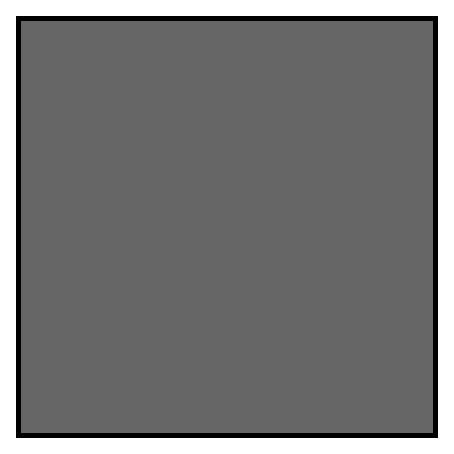
\includegraphics[width=0.5\textwidth]{example.eps}
%\caption{Please write your figure caption here}
%\label{fig:2}       % Give a unique label
%\end{figure*}


%\begin{acknowledgements}
%If you'd like to thank anyone, place your comments here
%and remove the percent signs.
%\end{acknowledgements}



\end{document}
% end of file template.tex

